
\chapter{Resultados}
\label{cha:resultados}

\begin{FraseCelebre}
  \begin{Frase}
    Cuando algo es lo suficientemente importante, lo haces incluso si las probabilidades no están a tu favor.
  \end{Frase}
  \begin{Fuente}
    Elon Musk
  \end{Fuente}
\end{FraseCelebre}

\section{Introducción}
\label{sec:intro-resultados}

En este capítulo se recogen los resultados obtenidos durante el diseño del sistema la detección de objetos abandonados. Para evaluar el funcionamiento de los distintos algoritmos que han sido empleados o diseñados es necesario realizar evaluaciones cuantitativas y cualitativas para validar su funcionamiento. En la detección de objetos, los investigadores evalúan sus algoritmos sobre los mismos datasets, de tal manera que se pueda contrastar los resultados con las propuestas de trabajos previos. Para evaluar un modelo de una red neuronal artificial se utilizan datasets de referencia para medir métricas de calidad para cuantificar el funcionamiento de los algoritmos.

Este capítulo está dividido en dos secciones diferenciadas. En la primera, se van a detallar las métricas de calidad que se han empleado para validar los datasets de referencia empleados en el entrenamiento de la red neuronal \gls{yolov4} y se expondrán los datasets empleados para evaluar los algoritmos que se han propuesto en el capítulo \ref{cha:desarrollo}. En la segunda, se expondrán y interpretarán los resultados obtenidos al ejecutar los algoritmos sobre los datasets descritos anteriormente.

\section{Entorno experimental}
\label{sec:desarrollo-resultados}

En el capítulo anterior se dijo que \gls{yolov4} está preentrenado sobre \gls{coco}. Sin embargo, durante las primeras pruebas de funcionamiento del detector de objetos se pudo observar que en la detección sobre los objetos de interés arrojaba en algunas ocasiones un \textit{confidence score} bajo dependiendo de la posición y ángulo que estuviera. \gls{yolov4} viene configurado por defecto con un \textit{threshold} sobre el \textit{confidence score} del 25\%, parámetro que se deberá de tener muy en cuenta más adelante. Por este motivo se ha decidido reentrenar la red sobre el dataset \gls{oidv4} con el objetivo de mejorar las métricas. Es por ello por lo que en el siguiente subapartado se va a hacer una introducción sobre las métricas más utilizadas en la evaluación de algoritmos de detección de objetos. Más adelante, en la sección \ref{subsec:metricas-calidad-openimagesv4} se visualizarán los resultados obtenidos tras el entrenamiento de la red.

\subsection{Métricas de calidad}
\label{subsec:metricas-calidad}

En esta sección se va a exponer las métricas de calidad \cite{padillaCITE2020} que han sido utilizadas para evaluar los datasets utilizados en el entrenamiento de \gls{yolov4}.

\subsubsection{Intersección sobre la unión (IoU)}
\label{subsubsec:iou}

\gls{iou} es una medida basada en el índice Jaccard que evalúa la superposición entre dos cuadros delimitadores. Requiere un cuadro delimitador de ground truth $B_{gt}$ y un cuadro delimitador de predicción $B_{p}$. Aplicando el \gls{iou} podemos saber si una detección es válida (verdadero positivo) o no (falso positivo).

El \gls{iou} viene dado por el área de superposición entre el cuadro delimitador de predicción y el cuadro delimitador de ground truth dividido por el área de unión entre ellos:

\begin{equation}
\label{eq:iou}
\text{IoU}=\frac{\text{area}\left(B_{p} \cap B_{gt} \right)}{\text{area}\left(B_{p} \cup B_{gt} \right)}    
\end{equation}

La siguiente figura ilustra el \gls{iou} entre un cuadro delimitador de ground truth (en verde) y un cuadro delimitador detectado (en rojo).

\begin{figure}[ht]
\centering
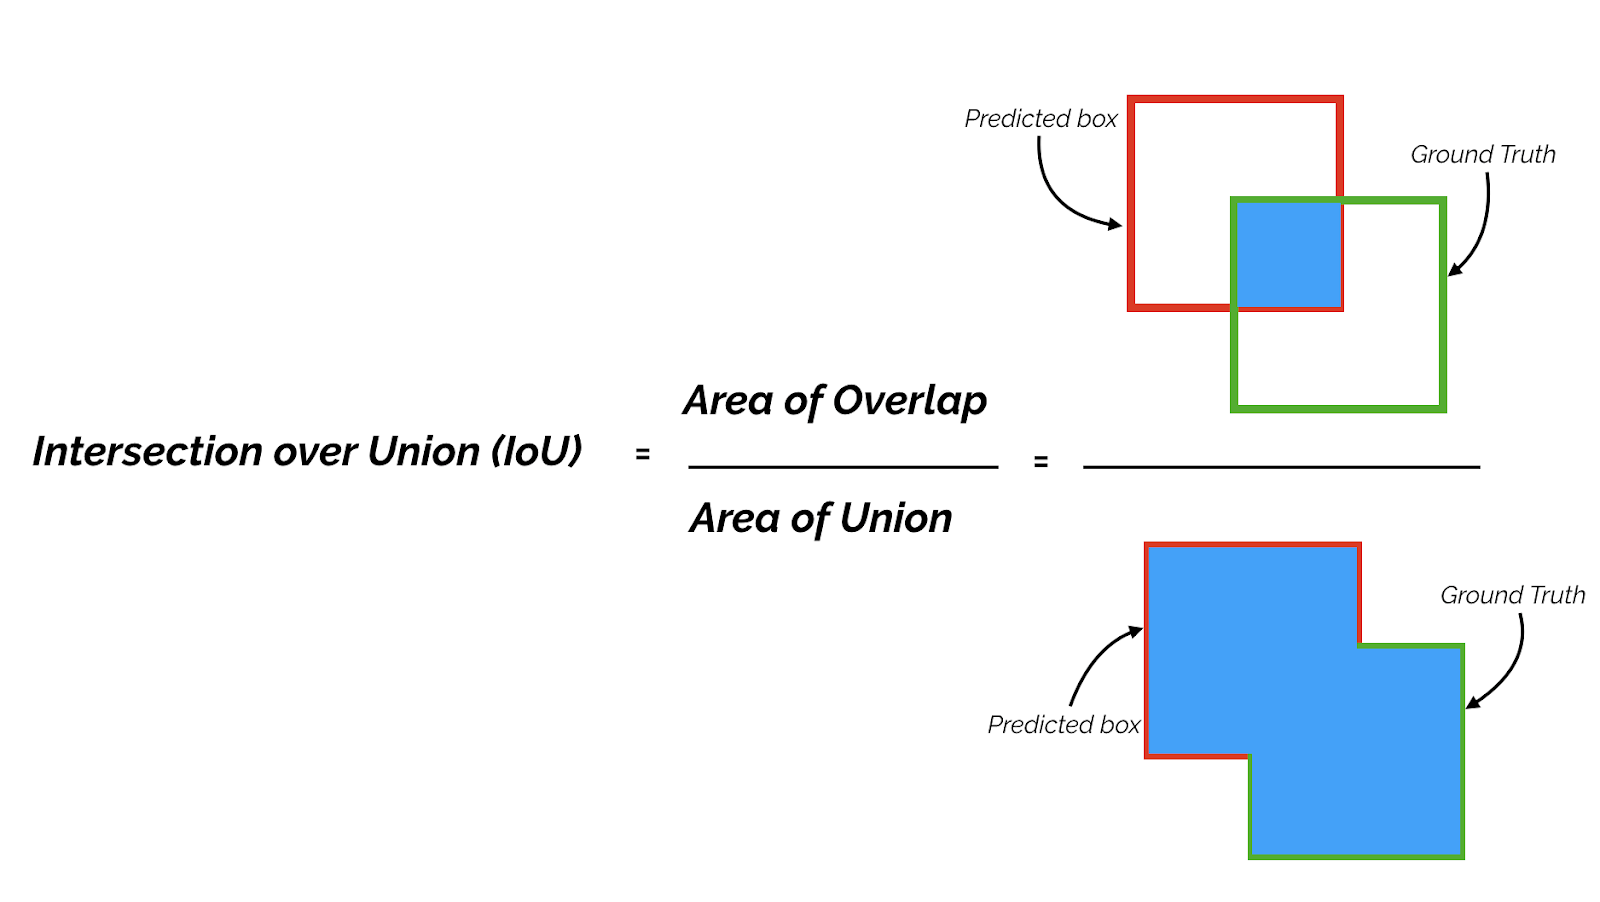
\includegraphics[width=0.45\textwidth]{img/chapters/resultados/metricas/iou.png}
\caption{\label{fig:iou}Área de superposición IoU entre los cuadros delimitadores \cite{padillaCITE2020}}
\end{figure}

\subsubsection{TP, TN, FP y FN}
\label{subsubsec:tp+tn+fp+fn}

Otros parámetros básicos en las métricas de calidad que conforman la matriz de confusión \cite{confusion-matrix} son:

\begin{itemize}
    \item \textbf{\gls{tp}}: Número de predicciones donde el clasificador predice correctamente la clase positiva como positiva. \gls{iou} $\geqslant$ \textit{threshold}
    \item \textbf{\gls{tn}}: Número de predicciones donde el clasificador predice correctamente la clase negativa como negativa. No se utiliza en el cálculo de métricas.
    \item \textbf{\gls{fp}}: Número de predicciones donde el clasificador predice incorrectamente la clase negativa como positiva. \gls{iou} <\ \textit{threshold}
    \item \textbf{\gls{fn}}: Número de predicciones donde el clasificador predice incorrectamente la clase positiva como negativa.
\end{itemize}

Típicamente el \textit{threshold} toma valores del 50\%, 75\% o 95\%.

\begin{figure}[ht]
\centering
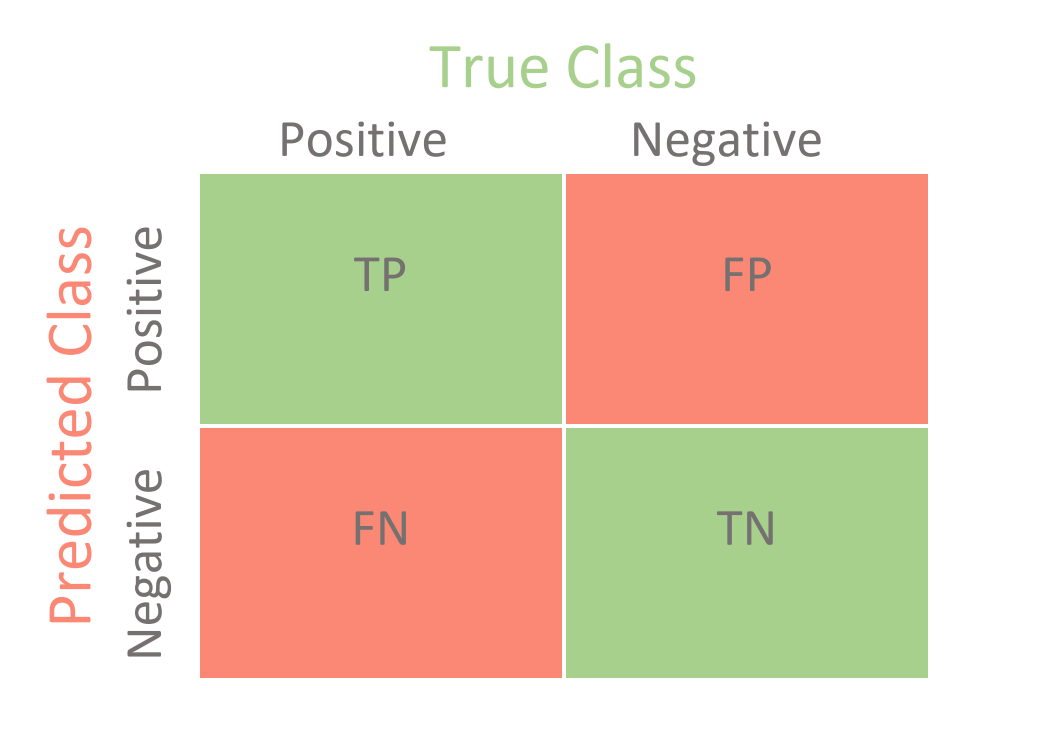
\includegraphics[width=0.45\textwidth]{img/chapters/resultados/metricas/confusion-matrix.png}
\caption{\label{fig:confusion-matrix}Matriz de confusión \cite{confusion-matrix}}
\end{figure}

\subsubsection{Precisión}
\label{subsubsec:precision}

La precisión es la capacidad de un modelo para identificar solo los objetos relevantes. Es el porcentaje de predicciones positivas correctas y viene dado por la siguiente expresión \ref{eq:precision}:

\begin{equation}
\label{eq:precision}
\text{P} = \frac{\text{TP}}{\text{TP}+\text{FP}}=\frac{\text{TP}}{\text{all detections}}
\end{equation}

\subsubsection{Recall}
\label{subsubsec:recall}

El Recall es la capacidad de un modelo para encontrar todos los casos relevantes (todos los cuadros delimitadores de ground truth). Es el porcentaje de verdadero positivo detectado entre todos los ground truths relevantes y viene dado por la siguiente expresión \ref{eq:recall}:

\begin{equation}
\label{eq:recall}
\text{R} = \frac{\text{TP}}{\text{TP}+\text{FN}}=\frac{\text{TP}}{\text{all ground truths}}
\end{equation}

\subsubsection{F-Score}
\label{subsubsec:f-score}

 El F-Score se trata de una medida estadística de precisión muy utilizada en las pruebas test de algoritmos. Es la media armónica que combina los valores de la precisión y el Recall. Viene dado por la expresión \ref{eq:f-score}:

\begin{equation}
\label{eq:f-score}
\text{F} = \frac{2 \cdotp \text{P} \cdotp \text{R}}{\text{P}+\text{R}}
\end{equation}

\subsubsection{Precisión media}
\label{subsubsec:averageprecision}

La precisión media es el valor medio de 11 puntos en la curva P-R para cada posible umbral (cada probabilidad de detección) para la misma clase (Precisión-Recall). En la ecuación \ref{eq:ap} se muestra el cálculo de la precisión media:

\begin{equation}
\label{eq:ap}
\text{AP}=\frac{1}{11} \sum_{r\in \left \{ 0, 0.1, ...,1 \right \}}\rho_{\text{interp}\left ( r \right )}
\end{equation}

con

$$\rho_{\text{interp}} = \max_{\tilde{r}:\tilde{r} \geq r} \rho\left ( \tilde{r} \right )$$

donde $\rho\left ( \tilde{r} \right )$ es la precisión medida en el Recall $\tilde{r}$

Por otro lado, el \gls{map} es la media de los \gls{ap} de todas las categorías de objetos. El \gls{map} se representa mediante la siguiente ecuación:

\begin{equation}
\label{eq:map}
\text{mAP} = \frac{1}{N} \sum_{i=1}^{N} \text{AP}_{1}
\end{equation}

\subsection{Datasets utilizados}
\label{subsec:datasets-utilizados}

Se van a describir los datasets más relevantes en la detección de objetos abandonados en los sistemas de videovigilancia así como los datasets de referencia sobre las que se validará previamente, en base a las métricas de calidad, el modelo entrenado o pre-entrenado utilizado.

En la tabla \ref{tab:datasets} se resumen los contenidos más relevantes de los datasets como son: número de secuencias, longitud media en minutos, escenario o tipo de desafío.

Los \textit{challenges} que se consideran de interés para la detección de objetos abandonados se numeran a continuación:

\begin{itemize}
    \item I = cambios de iluminación/sombras
    \item R = objetos alejados o pequeños
    \item P = personas estáticas en un punto durante un período de tiempo
    \item O = oclusiones
    \item LR = resolución vídeo baja
    \item RO = objetos abandonados o eliminados
\end{itemize}

\begin{table}[ht]
\centering
\caption{Datasets utilizados en la evaluación de los algoritmos}
\label{tab:datasets}
\begin{tabular}{lcccc}
\hline
\textbf{Nombre del dataset} & \textbf{\# Secuencias} & \textbf{\begin{tabular}[c]{@{}c@{}}Longitud media\\ (min)\end{tabular}} & \textbf{Escenario} & \textbf{Challenge} \\ \hline
PETS2007                    & 28                     & 1,96                                                                    & Aeropuerto         & I, R, P, O         \\
AVSSAB2007                  & 3                      & 3,46                                                                    & Estación de metro  & I, R, P, O         \\
GBA2018                     & 8                      & 0,74                                                                    & Interior           & I, R, P, O, RO     \\
ABODA                       & 11                     & 1,90                                                                    & Interior/exterior  & I, R, P, O         \\ \hline
\end{tabular}
\end{table}

\subsubsection{PETS2007 Dataset}

El dataset \gls{pets} \cite{pets2007-dataset} está formado por secuencias que contienen tres tipos escenarios con una complejidad ascendente: personas merodeando, robo de equipaje y equipaje desatendido/abandonado.

\paragraph*{Definición de merodear}\mbox{} \\
\label{parag:definicion-merodear}

Merodear se define como una persona que entra en escena y permanece dentro de la escena durante más de t segundos. Para los propósitos de \gls{pets}, 60 segundos.

\paragraph*{Definición de objeto desatendido}\mbox{} \\
\label{parag:definicion-desatendido-objeto}

Se utilizan tres reglas para determinar si el equipaje está atendido por parte de una persona o no:

\begin{itemize}
    \item Un equipaje es propiedad y es atendido por una persona o personas que ingresan al lugar con el equipaje hasta el punto en que el equipaje no está en contacto físico con la persona (regla contextual).
    \item En este punto, el equipaje es atendido por el propietario únicamente cuando se encuentran a una distancia de un metro del equipaje (regla espacial). Todas las distancias se miden entre los centroides del objeto en el plano del suelo (es decir, z = 0). Si una persona se encuentra a 2 metros de su equipaje, el sistema no debe activar ninguna alarma.
    \item Un equipaje está desatendido cuando el propietario está a más de 3 metros del equipaje. Si una persona cruza la línea de los 3 metros, el sistema debe usar la regla espacio-temporal el equipaje. Si el equipaje se encuentra en el rango de [2,3] metros se determina como una zona de advertencia.
\end{itemize}

\paragraph*{Definición de objeto abandonado}\mbox{} \\
\label{parag:definicion-abandono-objeto}

El abandono de una pieza de equipaje se define espacial y temporalmente. El abandono se define como:

Un bulto de equipaje que ha sido desatendido por el propietario por un período de 25 segundos consecutivos en el cual el propietario no ha vuelto a atender el equipaje, ni el equipaje ha sido atendido por una segunda persona. Si una pieza de equipaje se deja desatendida durante 25 segundos, se activa una alarma.

\paragraph*{Definición de robo de pieza de equipaje}\mbox{} \\
\label{parag:definicion-robo-pieza-equipaje}

El robo de una pieza de equipaje se define utilizando únicamente una restricción espacial. El robo se define como un artículo de equipaje movido a más de 3 metros del propietario. Se puede emitir una advertencia 2 metros del propietario.

\begin{figure}[ht]
  \centering
  \begin{subfigure}[b]{0.4\textwidth}
    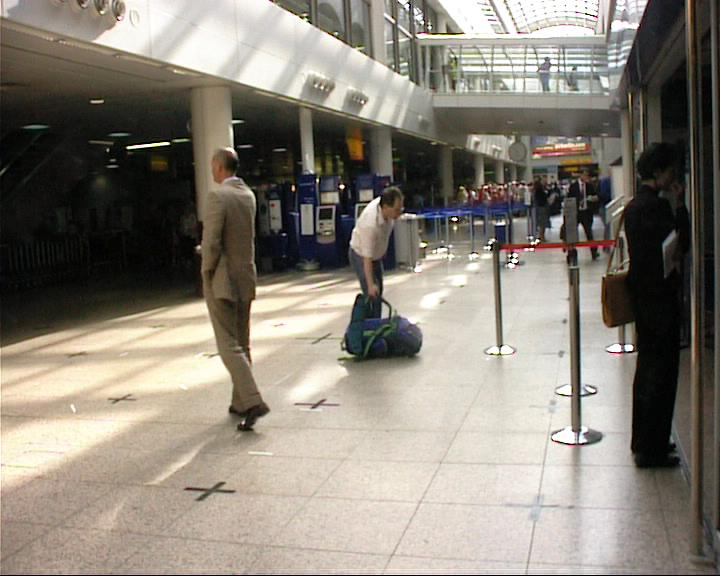
\includegraphics[width=\textwidth]{img/chapters/resultados/datasets/pets2007_1.jpg}
    \caption{}
    \label{fig:pets2007_1}
  \end{subfigure}
  \qquad\qquad
  \begin{subfigure}[b]{0.4\textwidth}
    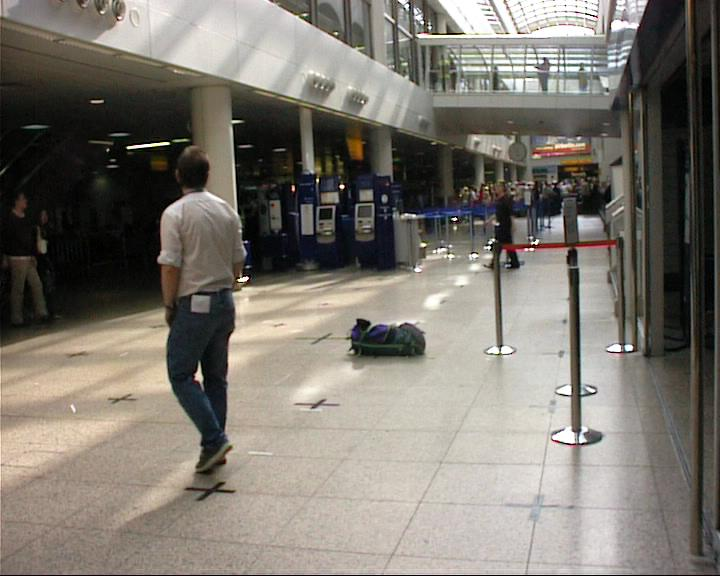
\includegraphics[width=\textwidth]{img/chapters/resultados/datasets/pets2007_2.jpg}
    \caption{}
    \label{fig:pets2007_2}
  \end{subfigure}
  \caption{Imágenes extraídas del dataset PETS2007 \cite{pets2007-dataset}.
    (\protect\subref{fig:pets2007_1}) Fotograma de la secuencia S08-camera4 donde un hombre deja su equipaje en el suelo.
    (\protect\subref{fig:pets2007_2}) Otro fotograma de la secuencia S08-camera4 donde el hombre abandona el lugar sin su equipaje.}
  \label{fig:pets2007_S08}
\end{figure}

Las cámaras utilizadas para la grabación de las distintas secuencias son las siguientes:

\begin{itemize}
    \item Cámara 1: Canon MV-1 1xCCD w/progressive scan
    \item Cámara 2: Sony DCR-PC1000E 3xCMOS
    \item Cámara 3: Canon MV-1 1xCCD w/progressive scan
    \item Cámara 4: Sony DCR-PC1000E 3xCMOS
\end{itemize}


La resolución de todas las secuencias es PAL standard (768 x 576 píxeles y 25 \gls{fps}) y comprimidas como secuencias de imágenes JPEG (aprox. 90\% de calidad).

\begin{figure}[ht]
  \centering
  \begin{subfigure}[b]{0.4\textwidth}
    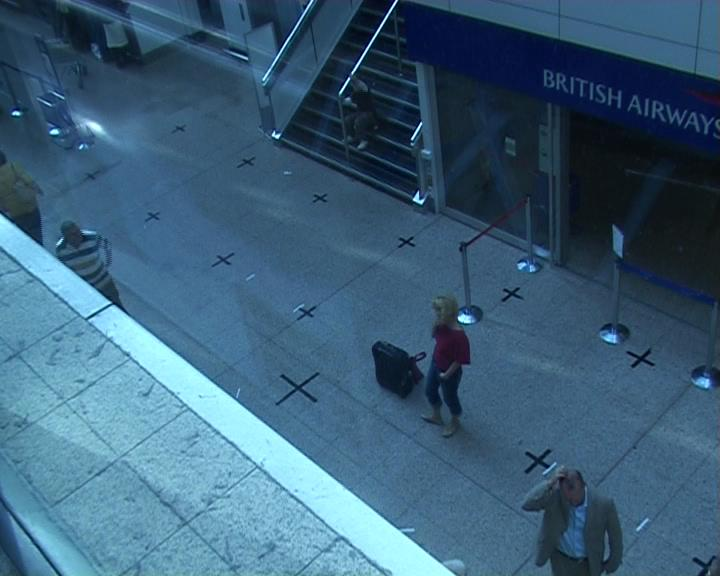
\includegraphics[width=\textwidth]{img/chapters/resultados/datasets/pets2007_3.jpg}
    \caption{}
    \label{fig:pets2007_3}
  \end{subfigure}
  \qquad\qquad
  \begin{subfigure}[b]{0.4\textwidth}
    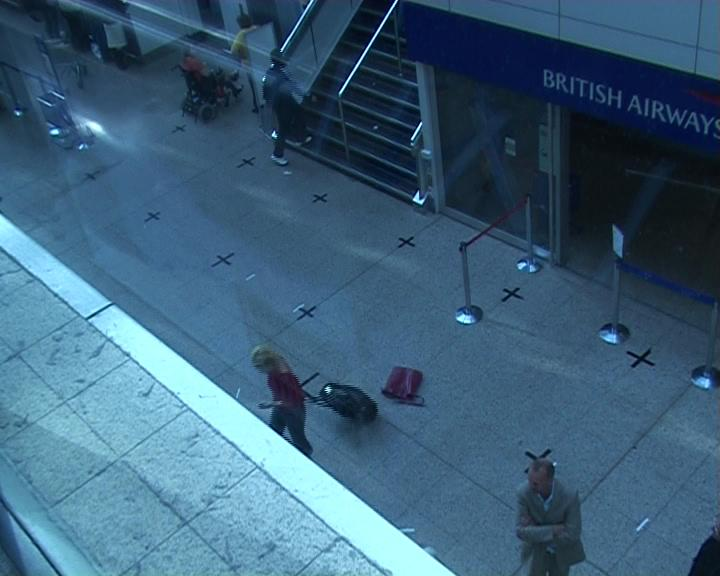
\includegraphics[width=\textwidth]{img/chapters/resultados/datasets/pets2007_4.jpg}
    \caption{}
    \label{fig:pets2007_4}
  \end{subfigure}
  \caption{Imágenes extraídas del dataset PETS2007 \cite{pets2007-dataset}.
    (\protect\subref{fig:pets2007_3}) Fotograma de la secuencia S07-thirdView donde una mujer se encuentra junto a su equipaje.
    (\protect\subref{fig:pets2007_4}) Otro fotograma de la secuencia S07-thirdView donde la mujer abandona el lugar sin su bolso.}
  \label{fig:pets2007_S07}
\end{figure}

En este proyecto solo se va a tener en cuenta tener en cuenta cuando un equipaje ha sido abandonado sin propietario en un tiempo superior a 15 segundos o cuando ha sido desatendido por su propietario alejándose más de 5 veces la distancia que se establece en el momento de la asociación persona-objeto.

\subsubsection{AVSSAB2007 Dataset}

\gls{avss} \cite{AVSSAB2007-dataset} es un subconjunto de datos del dataset AVSS 2007, el cual fue creado para el \textit{i-LIDS bag and vehicle detection challenge} que se celebró en la 14\textsuperscript{th} IEEE International Conference on Advanced Video and Signal based Surveillance en septiembre de 2007. En ella se tenía como objetivo atraer artículos del Estado del Arte para presentar metodologías para la detección de eventos. Tiene la intención de informar sobre la precisión, solidez y complejidad de las secuencias de vídeo del dataset.

Se ha utilizado el subconjunto de secuencias dedicadas a la detección de objetos abandonados. Este subdataset está formado por tres secuencias de vídeo grabadas a una resolución de 720 x 576 píxeles a 25 \gls{fps}. El modelo de la cámara no se especifica.

El \gls{roi} está divido en tres zonas: cercana, media, lejos. En cada una de las secuencias de vídeo el objeto que es abandonado se encuentra en cada una de las zonas que se muestran en la figura \ref{fig:avssab2007-zones}.

\begin{figure}[ht]
\centering
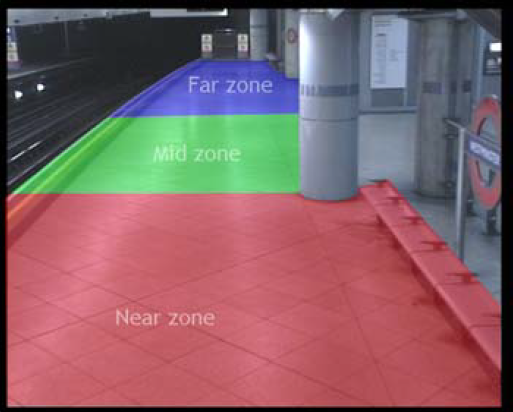
\includegraphics[width=0.4\textwidth]{img/chapters/resultados/datasets/avssab2007-zones.png}
\caption{\label{fig:avssab2007-zones}Regiones de interés del dataset AVSSAB2007 \cite{AVSSAB2007-dataset}}
\end{figure}

Todas las secuencias presentan la misma estructura en la sucesión de eventos:

\begin{itemize}
    \item Una persona ha colocado un objeto que estaba en su posesión en una de las áreas de detección
    \item Esa persona abandona el área de detección sin el objeto
    \item Esa persona aún no ha regresado al objeto más de 60 segundos después de haber abandonado el área de detección
    \item El objeto permanece en el área de detección hasta finalizar la secuencia de vídeo
\end{itemize}

\begin{figure}[ht]
  \centering
  \begin{subfigure}[b]{0.4\textwidth}
    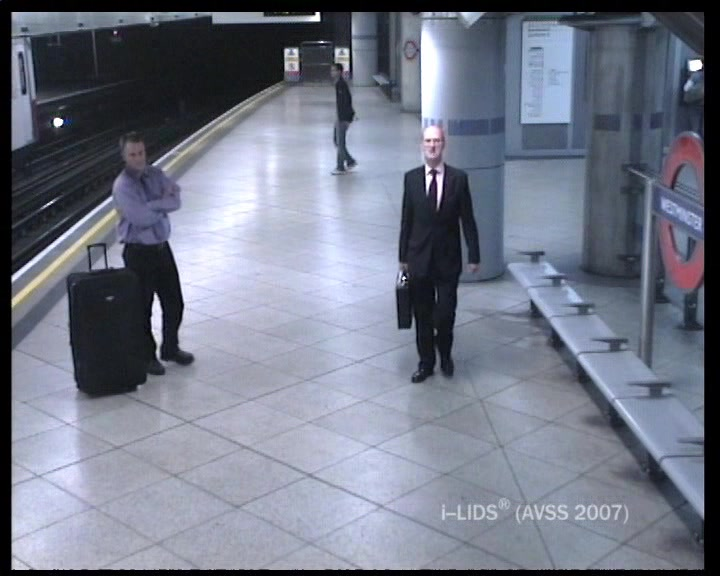
\includegraphics[width=\textwidth]{img/chapters/resultados/datasets/AVSSAB_1.jpg}
    \caption{}
    \label{fig:avssab2007_1}
  \end{subfigure}
  \qquad\qquad
  \begin{subfigure}[b]{0.4\textwidth}
    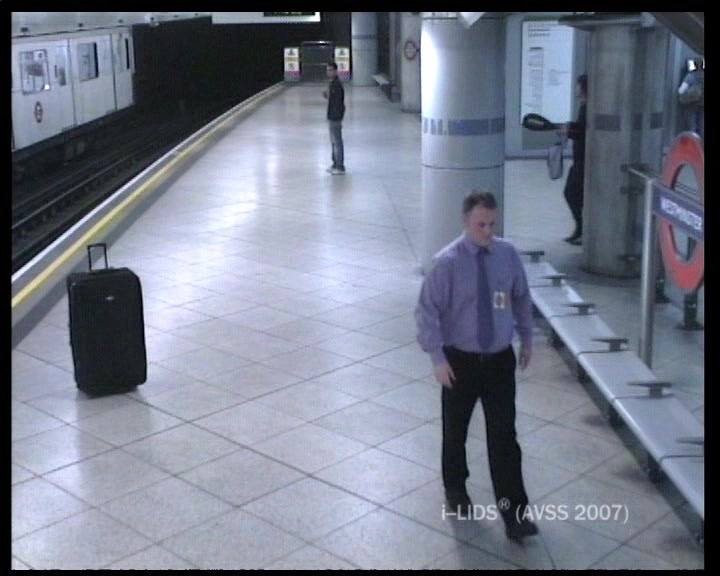
\includegraphics[width=\textwidth]{img/chapters/resultados/datasets/AVSSAB_2.jpg}
    \caption{}
    \label{fig:avssab2007_2}
  \end{subfigure}
  \caption{Imágenes extraídas del dataset AVSSAB2007 \cite{AVSSAB2007-dataset}.
    (\protect\subref{fig:avssab2007_1}) Fotograma de la secuencia AVSSAB-Easy donde el hombre abandona su maleta en la zona cercana.
    (\protect\subref{fig:avssab2007_2}) Fotograma de la secuencia AVSSAB-Medium donde una mujer se encuentra junto a su bolsa de mano en la zona media del andén del metro.}
  \label{fig:avssab2007_near_medium}
\end{figure}

\subsubsection{GBA2018 Dataset}

El dataset \gls{gba2018} \cite{gba-dataset} fue grabado y etiquetado por el grupo de investigación \gls{geintra} en la \gls{eps} de la \gls{uah} durante la realización del \gls{tfm} de David Valdivieso López \cite{valdivieso2018}. Está orientado a la evaluación de algoritmos de detección de objetos abandonados y eventos anómalos como estampidas. El dataset está formado 8 secuencias en 2 escenarios distintos grabadas con una GoPro HERO4 a una resolución de 1920 x 1080 píxeles a 60 \gls{fps}.

\begin{figure}[ht]
\centering
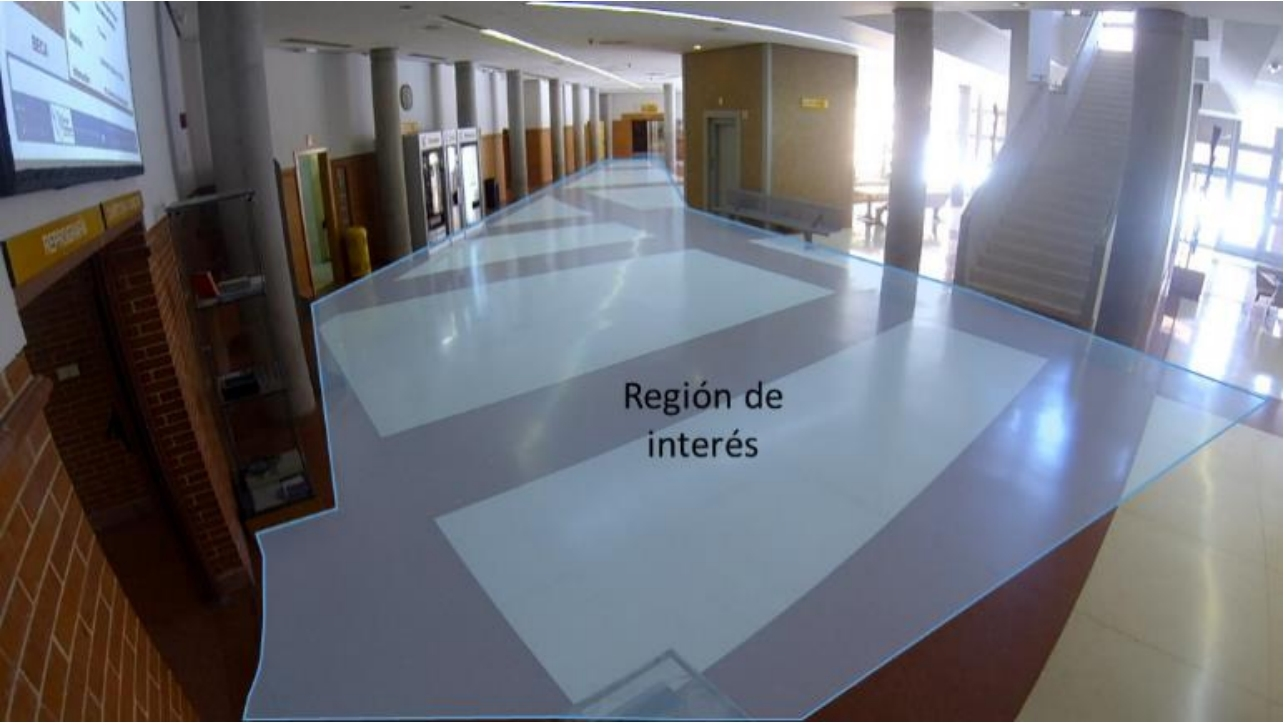
\includegraphics[width=0.4\textwidth]{img/chapters/resultados/datasets/hall-eps.jpg}
\caption{\label{fig:roi-hall-eps}ROI del hall de la Escuela Politécnica Superior (UAH) \cite{7743617}}
\end{figure}

En el primer escenario se muestra como \gls{roi} el hall de la \gls{eps} desde un plano alejado donde ocurren eventos como abandono de maletas, mochilas y bolsas de mano. Se trata de un escenario complejo ya que hay cambios tanto de luz natural como artificial y personas y objetos situados a distancias largas, lo que puede dificultar la tarea de detección.

\begin{figure}[ht!]
  \centering
  \begin{subfigure}[b]{0.4\textwidth}
    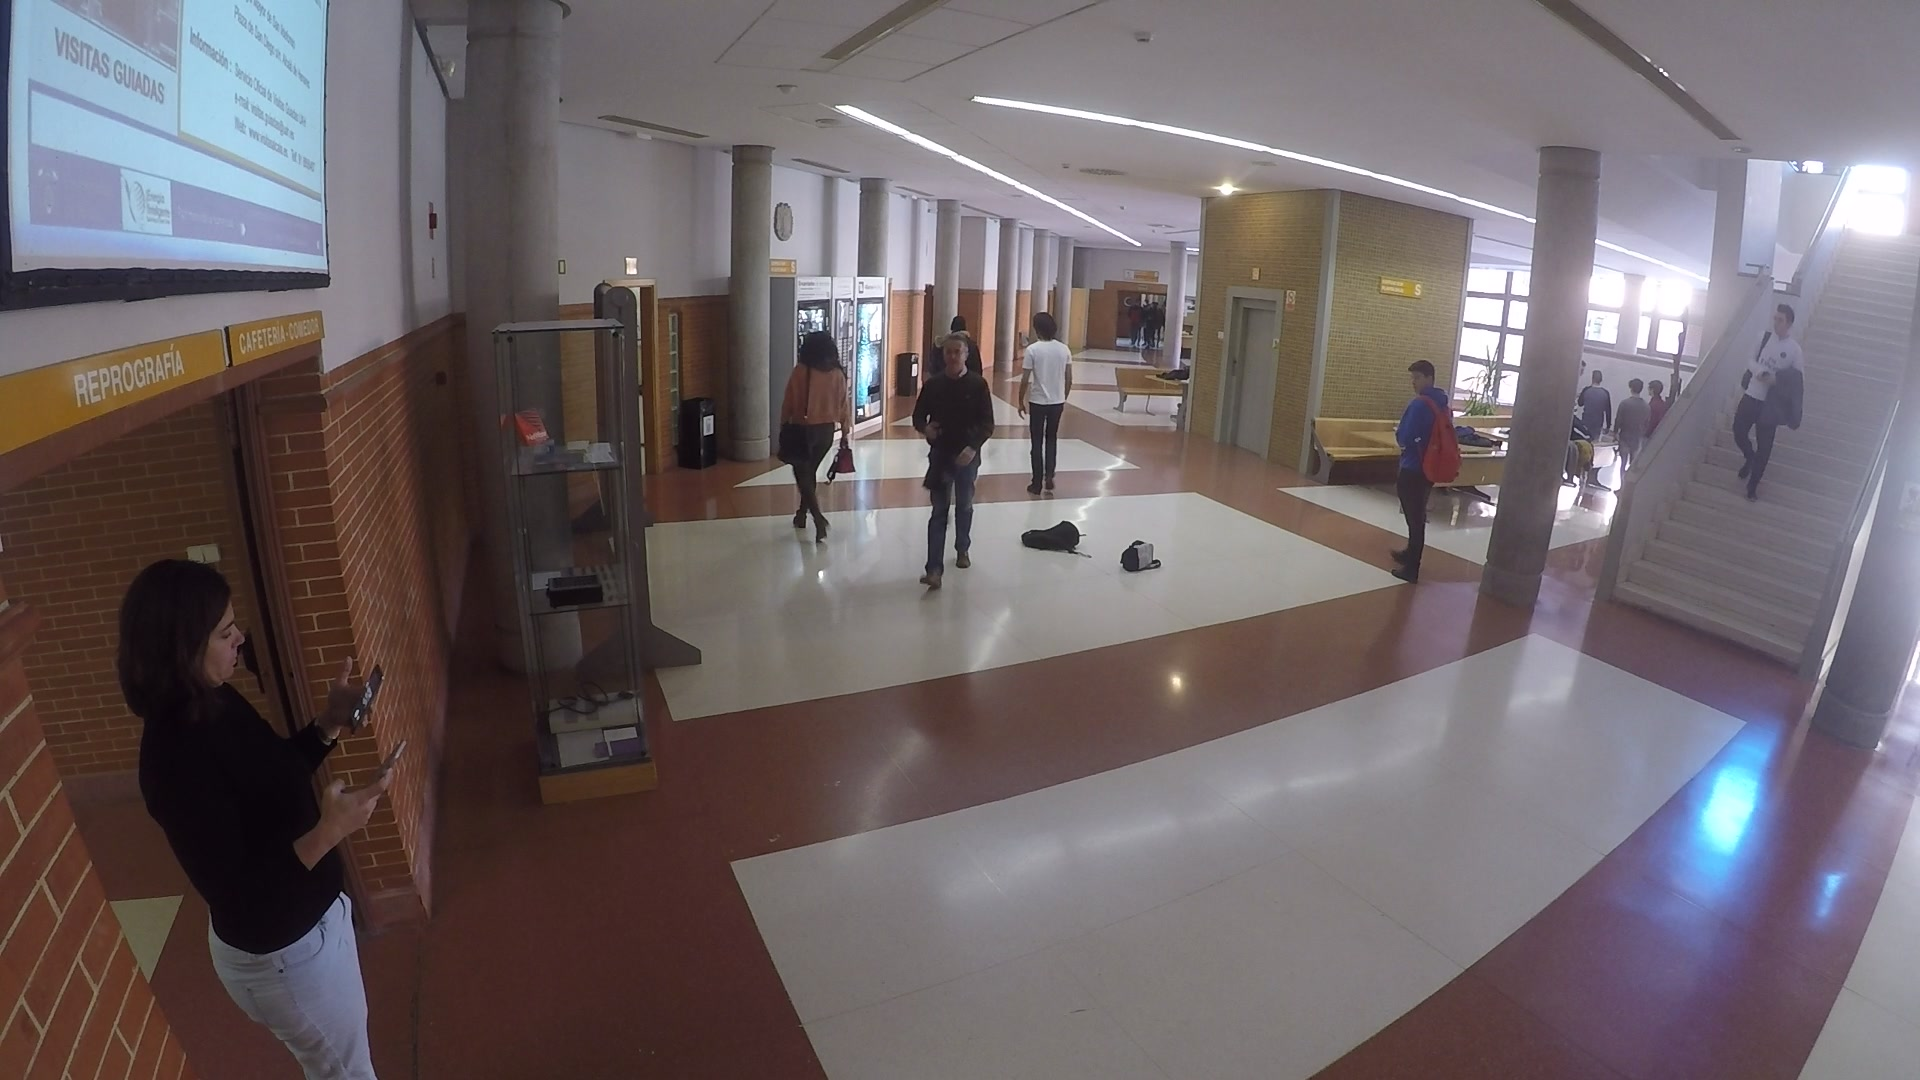
\includegraphics[width=\textwidth]{img/chapters/resultados/datasets/GBA_1.jpg}
    \caption{}
    \label{fig:GBA_1}
  \end{subfigure}
  \qquad\qquad
  \begin{subfigure}[b]{0.4\textwidth}
    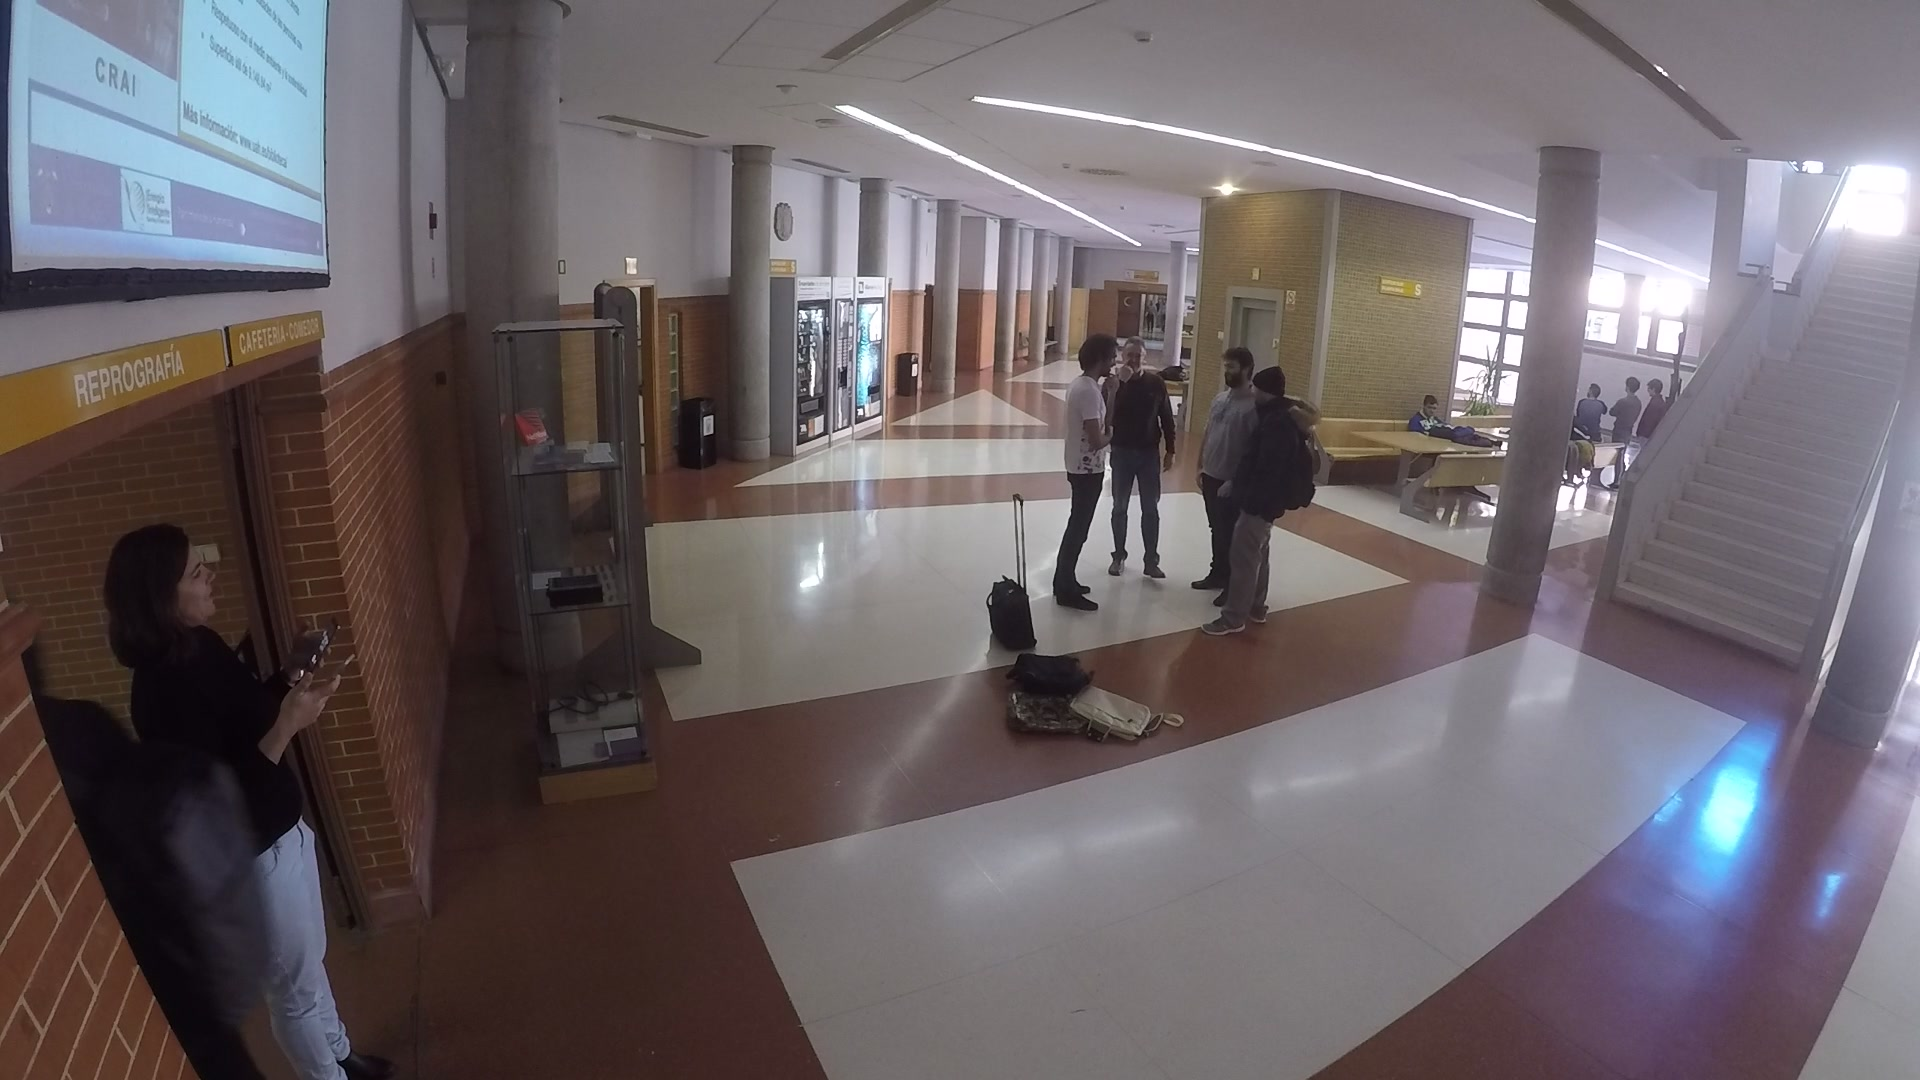
\includegraphics[width=\textwidth]{img/chapters/resultados/datasets/GBA_2.jpg}
    \caption{}
    \label{fig:GBA_2}
  \end{subfigure}
  \caption{Imágenes extraídas de secuencias del primer escenario del dataset GBA2018 \cite{gba-dataset}.
    (\protect\subref{fig:GBA_1}) Fotograma de la secuencia GBA-far-video2 donde dos bolsas de mano han sido abandonadas en medio del hall.
    (\protect\subref{fig:GBA_2}) Fotograma de la secuencia GBA-far-video3 donde varias bolsas y maletas están alejadas de sus propietarios.}
  \label{fig:GBA1}
\end{figure}

El \gls{roi} del segundo escenario se encuentra en el pasillo que conecta el hall con la cafetería. El plano de grabación es más cercano respecto al anterior con lo que se consideran secuencias más fáciles de evaluar ya que no se encuentran elementos de interés alejados ni tampoco hay cambios bruscos en la iluminación.

\begin{figure}[ht]
  \centering
  \begin{subfigure}[b]{0.4\textwidth}
    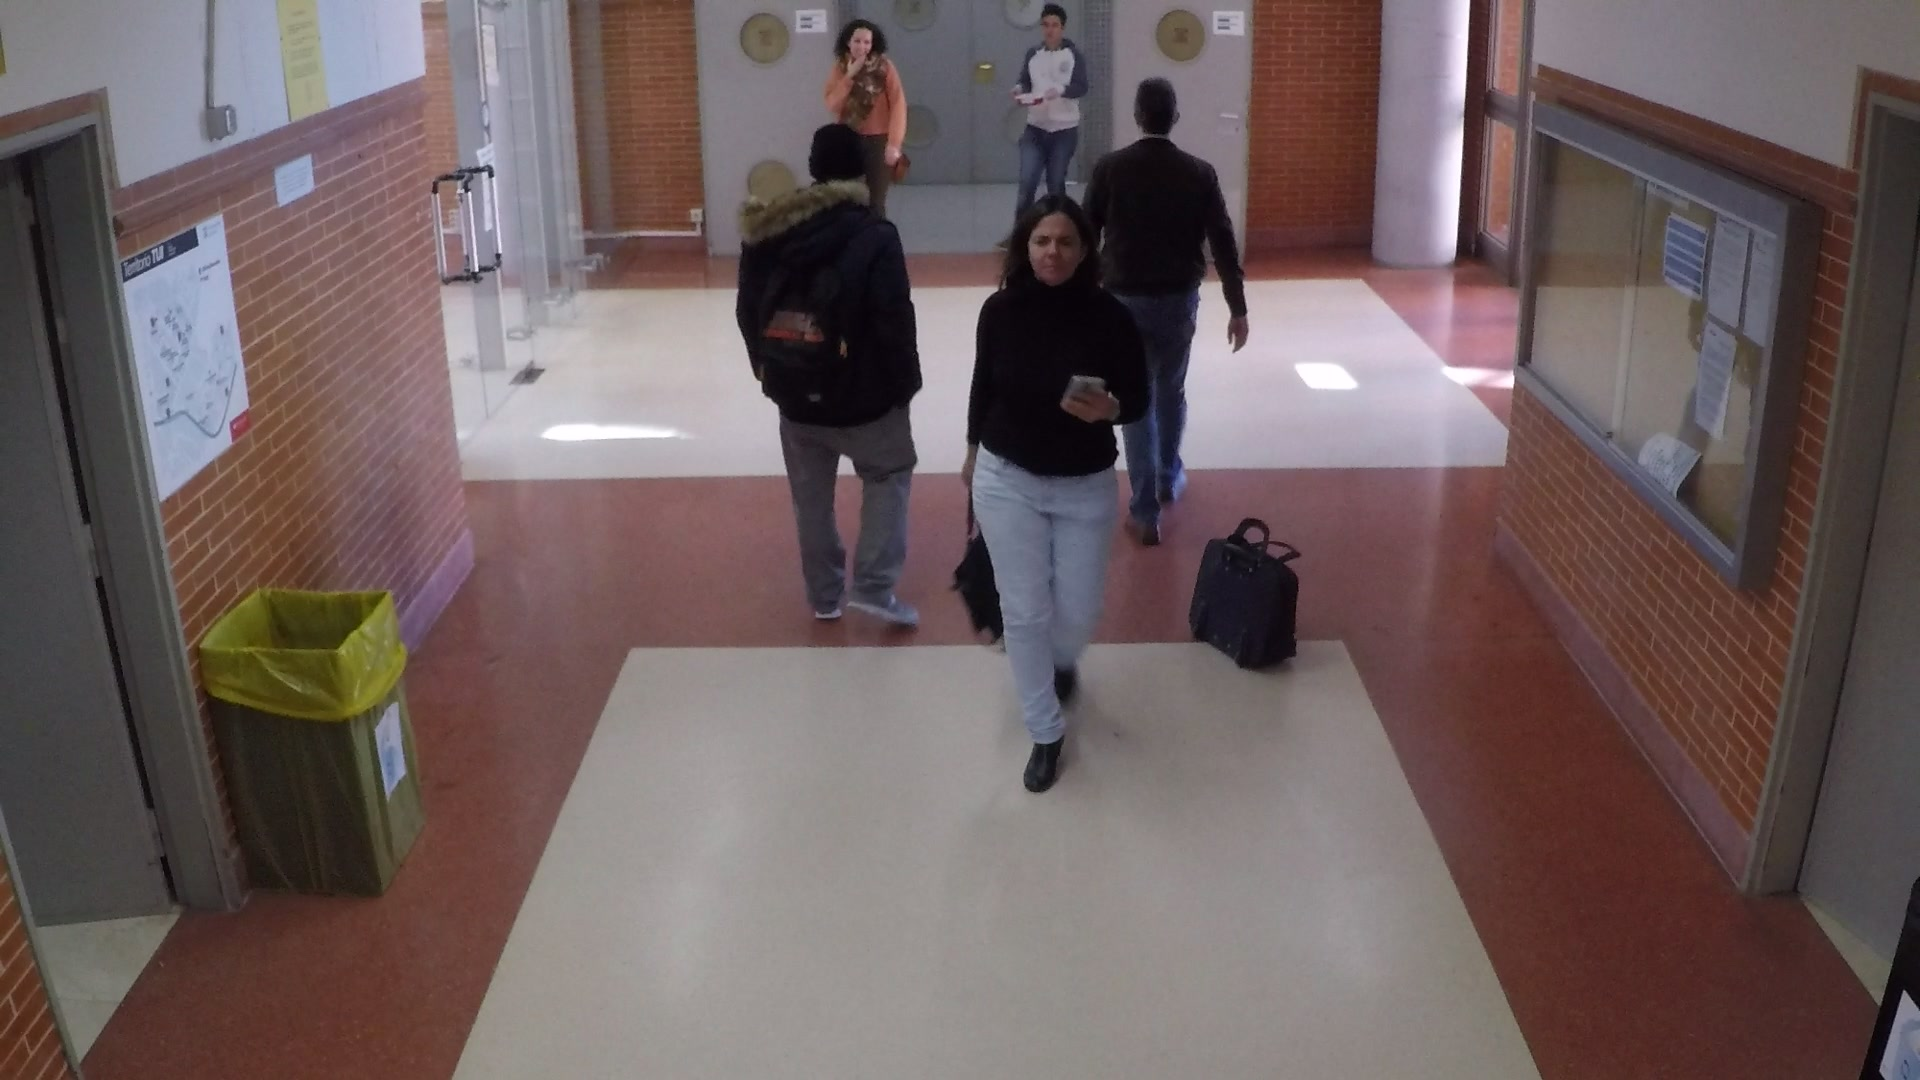
\includegraphics[width=\textwidth]{img/chapters/resultados/datasets/GBA_3.jpg}
    \caption{}
    \label{fig:GBA_3}
  \end{subfigure}
  \qquad\qquad
  \begin{subfigure}[b]{0.4\textwidth}
    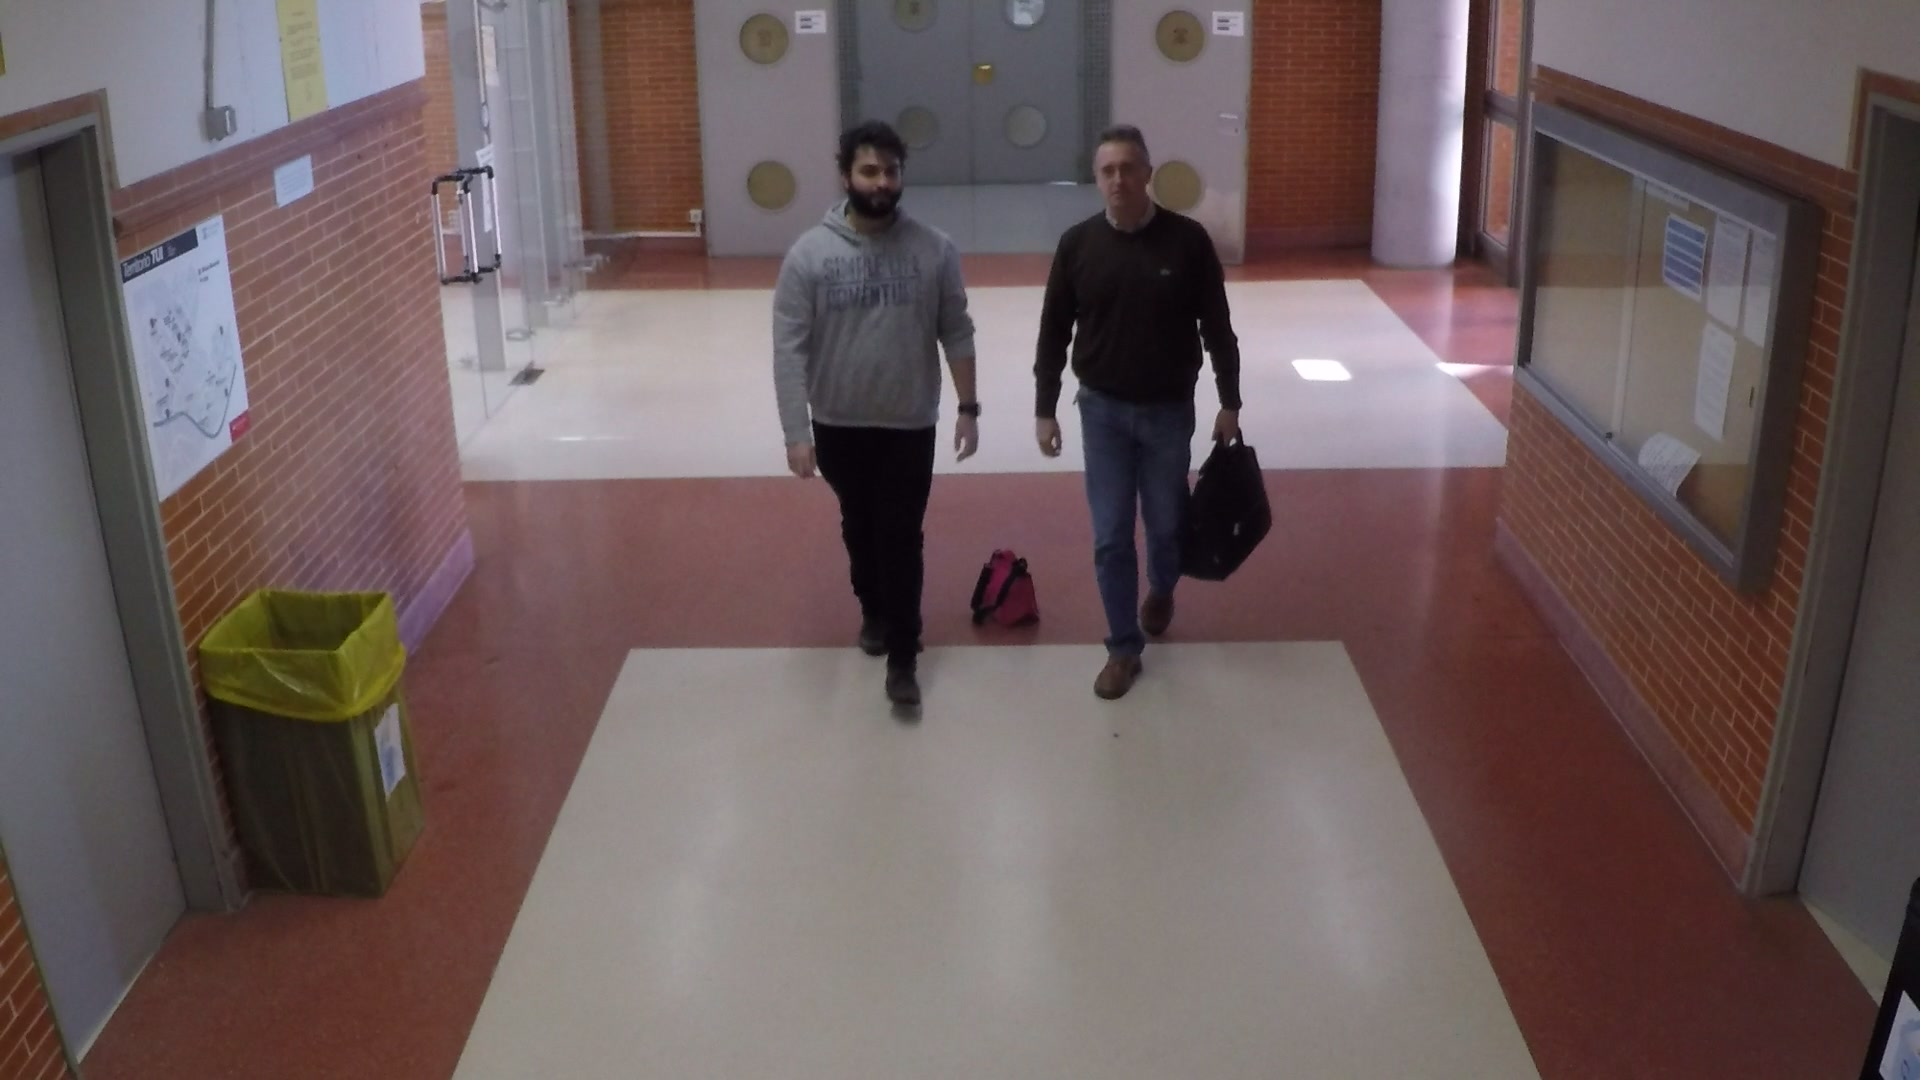
\includegraphics[width=\textwidth]{img/chapters/resultados/datasets/GBA_4.jpg}
    \caption{}
    \label{fig:GBA_4}
  \end{subfigure}
  \caption{Imágenes extraídas de secuencias del segundo escenario del dataset GBA2018 \cite{gba-dataset}.
    (\protect\subref{fig:GBA_3}) Fotograma de la secuencia GBA-near-big-video2 donde una bolsa de mano es abandonada en el pasillo de la cafetería.
    (\protect\subref{fig:GBA_4}) Fotograma de la secuencia GBA-near-big-video4 donde dos personas abandonan una pequeña bolsa de mano.}
  \label{fig:GBA2}
\end{figure}

\subsubsection{ABODA Dataset}

\gls{aboda} \cite{aboda-dataset} es un dataset propuesto por primera vez en 2015 para la detección de objetos abandonados. \gls{aboda} está formado por 11 secuencias etiquetadas con varios escenarios de aplicaciones reales que son un desafío para la detección de objetos abandonados. Las situaciones incluyen escenas de gran aglomeración de personas, cambios en las condiciones de iluminación, detección nocturna, así como ambientes interiores y exteriores.

Algunas secuencias de vídeo están grabadas a resoluciones: de 720 x 480 píxeles a 30 \gls{fps}, y otras secuencias a 640 x 480 píxeles y 30 \gls{fps}. El modelo de la cámara no se especifica.

La figura \ref{fig:aboda1} muestra los fotogramas de vídeo1 grabados en un entorno interior con luz artificial. En esta secuencia dos personas están interactuando entre sí y una persona tiene una bolsa (Fig. \ref{fig:aboda_1}). Más tarde, una de las dos personas deja caer su bolso y ambos abandonan el lugar ((Fig. \ref{fig:aboda_2}))

\begin{figure}[ht]
  \centering
  \begin{subfigure}[b]{0.4\textwidth}
    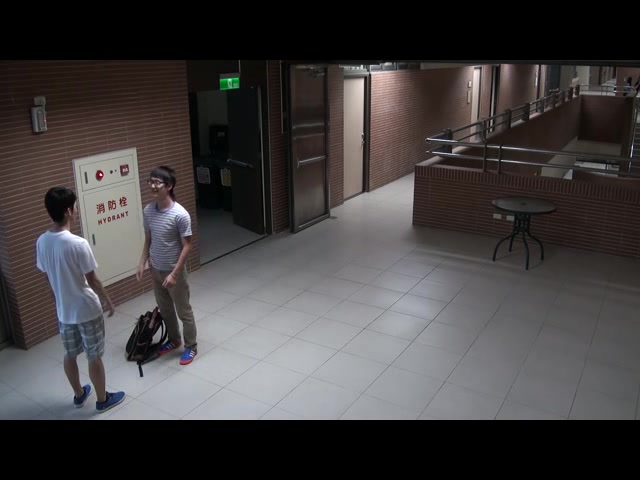
\includegraphics[width=\textwidth]{img/chapters/resultados/datasets/aboda_1.jpg}
    \caption{}
    \label{fig:aboda_1}
  \end{subfigure}
  \qquad\qquad
  \begin{subfigure}[b]{0.4\textwidth}
    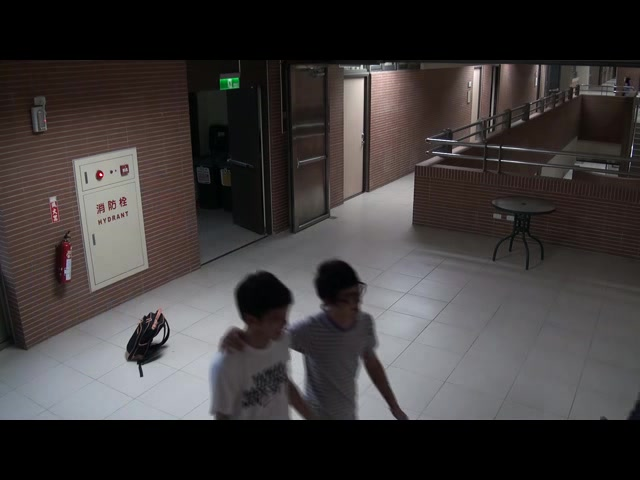
\includegraphics[width=\textwidth]{img/chapters/resultados/datasets/aboda_2.jpg}
    \caption{}
    \label{fig:aboda_2}
  \end{subfigure}
  \caption{Imágenes extraídas del dataset ABODA \cite{aboda-dataset}.
    (\protect\subref{fig:aboda_1}) Fotograma donde dos chicos conversan en el hall.
    (\protect\subref{fig:aboda_2}) Otro fotograma donde los dos chicos abandonan una mochila.}
  \label{fig:aboda1}
\end{figure}

Este dataset también incluye escenas de aglomeración de personas que se encuentran en aeropuertos o estaciones de tren, iluminación variable de día y grabaciones nocturnas.

\begin{figure}[ht]
  \centering
  \begin{subfigure}[b]{0.4\textwidth}
    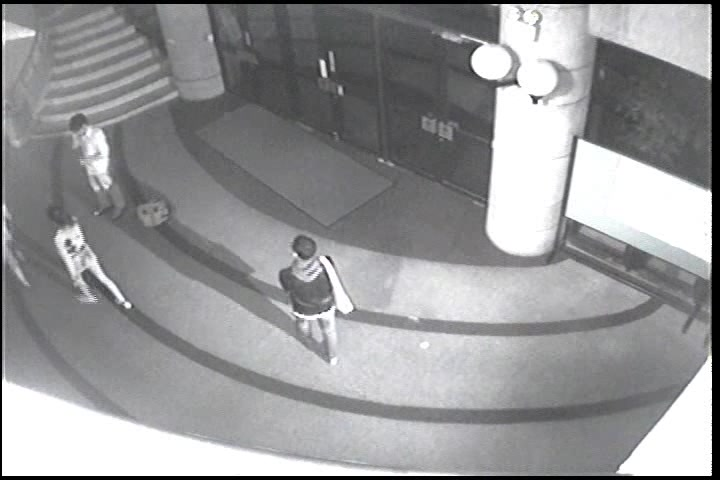
\includegraphics[width=\textwidth]{img/chapters/resultados/datasets/aboda_3.jpg}
    \caption{}
    \label{fig:aboda_3}
  \end{subfigure}
  \qquad\qquad
  \begin{subfigure}[b]{0.4\textwidth}
    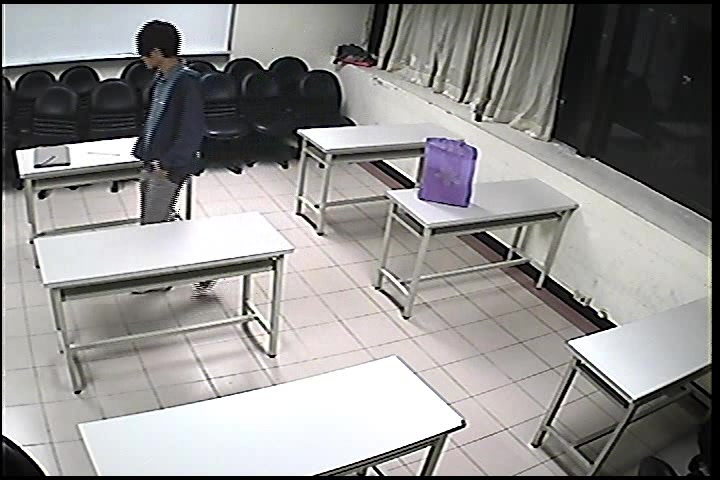
\includegraphics[width=\textwidth]{img/chapters/resultados/datasets/aboda_4.jpg}
    \caption{}
    \label{fig:aboda_4}
  \end{subfigure}
  \caption{Imágenes extraídas del dataset ABODA \cite{aboda-dataset}.
    (\protect\subref{fig:aboda_3}) Fotograma de la secuencia video5 de una grabación nocturna.
    (\protect\subref{fig:aboda_4}) Fotograma de la secuencia video11 donde hay varias personas haciendo cola en un aeropuerto.}
  \label{fig:aboda2}
\end{figure}

\section{Resultados experimentales}
\label{sec:resultados-experimentales}

Una vez elegido \gls{coco} como dataset de referencia para usar con \gls{yolov4}, se va a ver los resultados obtenidos en distintos algoritmos.

\textcolor{red}{Hacer introducción donde se explique que primero se va a relizar una evaluación cuantitativa de los entrenamientos de las redes neuronales y después una evaluación cualitativa del funcionamiento de los algoritmos}

\subsection{Métricas de calidad en Open Image Dataset v4}
\label{subsec:metricas-calidad-openimagesv4}

En la tabla \ref{tab:metricas-test1_1}, \ref{tab:metricas-test1_2}, \ref{tab:metricas-test1_3} y \ref{tab:metricas-test1_4} se reflejan las métricas más relevantes cada 1000 iteraciones del entrenamiento de la red neuronal.

\begin{table}[ht]
\centering
\caption{Métricas de calidad en el primer entrenamiento con OIDv4 [1]}
\label{tab:metricas-test1_1}
\begin{tabular}{lcccc}
\hline
\textbf{Iterations} & \textbf{\begin{tabular}[c]{@{}c@{}}AP person\\ (\%)\end{tabular}} & \textbf{\begin{tabular}[c]{@{}c@{}}AP handbag\\ (\%)\end{tabular}} & \textbf{\begin{tabular}[c]{@{}c@{}}AP backpack\\ (\%)\end{tabular}} & \textbf{\begin{tabular}[c]{@{}c@{}}AP suitcase\\ (\%)\end{tabular}} \\ \hline
1.000               & 31,26                                                             & 85,45                                                              & 67,99                                                               & 42,15                                                               \\
\textbf{2.000}      & \textbf{43,96}                                                    & \textbf{92,39}                                                     & \textbf{63,88}                                                      & \textbf{64,79}                                                      \\
3.000               & 36,16                                                             & 90,10                                                              & 67,88                                                               & 53,33                                                               \\
4.000               & 35,56                                                             & 91,99                                                              & 64,61                                                               & 57,74                                                               \\
5.000               & 34,21                                                             & 87,35                                                              & 68,73                                                               & 48,77                                                               \\
6.000               & 36,74                                                             & 89,48                                                              & 65,83                                                               & 49,09                                                               \\
7.000               & 34,76                                                             & 88,94                                                              & 68,20                                                               & 51,24                                                               \\
8.000               & 38,30                                                             & 87,69                                                              & 72,00                                                               & 58,89                                                               \\ \hline
\end{tabular}
\end{table}

\begin{table}[ht]
\centering
\caption{Métricas de calidad en el primer entrenamiento con OIDv4 [2]}
\label{tab:metricas-test1_2}
\begin{tabular}{lcccc}
\hline
\textbf{Iterations} & \textbf{TP person} & \textbf{TP handbag} & \textbf{TP backpack} & \textbf{TP suitcase} \\ \hline
1.000               & 249                & 52                  & 19                   & 16                   \\
\textbf{2.000}      & \textbf{338}       & \textbf{54}         & \textbf{19}          & \textbf{19}          \\
3.000               & 324                & 54                  & 21                   & 18                   \\
4.000               & 329                & 54                  & 20                   & 20                   \\
5.000               & 313                & 50                  & 23                   & 16                   \\
6.000               & 323                & 52                  & 20                   & 13                   \\
7.000               & 288                & 53                  & 19                   & 18                   \\
8.000               & 308                & 49                  & 21                   & 19                   \\ \hline
\end{tabular}
\end{table}

\begin{table}[ht]
\centering
\caption{Métricas de calidad en el primer entrenamiento con OIDv4 [3]}
\label{tab:metricas-test1_3}
\begin{tabular}{lcccc}
\hline
\textbf{Iterations} & \textbf{FP person} & \textbf{FP handbag} & \textbf{FP backpack} & \textbf{FP suitcase} \\ \hline
1.000               & 416                & 20                  & 11                   & 42                   \\
\textbf{2.000}      & \textbf{489}       & \textbf{15}         & \textbf{16}          & \textbf{7}           \\
3.000               & 479                & 22                  & 18                   & 36                   \\
4.000               & 521                & 10                  & 20                   & 19                   \\
5.000               & 474                & 14                  & 19                   & 22                   \\
6.000               & 446                & 7                   & 14                   & 13                   \\
7.000               & 391                & 19                  & 13                   & 16                   \\
8.000               & 412                & 11                  & 16                   & 17                   \\ \hline
\end{tabular}
\end{table}

\begin{table}[ht!]
\centering
\caption{Métricas de calidad en el primer entrenamiento con OIDv4 [4]}
\label{tab:metricas-test1_4}
\begin{tabular}{lcccccccc}
\hline
\textbf{Iterations} & \textbf{TP}  & \textbf{FP}  & \textbf{FN}  & \textbf{\begin{tabular}[c]{@{}c@{}}Precision\\ (\%)\end{tabular}} & \textbf{\begin{tabular}[c]{@{}c@{}}Recall\\ (\%)\end{tabular}} & \textbf{\begin{tabular}[c]{@{}c@{}}F-score\\ (\%)\end{tabular}} & \textbf{\begin{tabular}[c]{@{}c@{}}Average IoU\\ (\%)\end{tabular}} & \textbf{\begin{tabular}[c]{@{}c@{}}mAP @ 0.5\\ (\%)\end{tabular}} \\ \hline
1.000               & 336          & 489          & 367          & 40,73                                                             & 47,80                                                          & 43,98                                                           & 29,36                                                               & 56,71                                                             \\
\textbf{2.000}      & \textbf{430} & \textbf{527} & \textbf{273} & \textbf{44,93}                                                    & \textbf{61,17}                                                 & \textbf{51,81}                                                  & \textbf{34,13}                                                      & \textbf{66,25}                                                    \\
3.000               & 417          & 555          & 286          & 42,90                                                             & 59,32                                                          & 49,79                                                           & 32,29                                                               & 61,87                                                             \\
4.000               & 423          & 570          & 280          & 42,60                                                             & 60,17                                                          & 49,88                                                           & 33,30                                                               & 62,47                                                             \\
5.000               & 402          & 529          & 301          & 43,18                                                             & 57,18                                                          & 49,20                                                           & 32,53                                                               & 59,77                                                             \\
6.000               & 408          & 480          & 295          & 45,95                                                             & 58,04                                                          & 51,29                                                           & 36,76                                                               & 60,28                                                             \\
7.000               & 378          & 439          & 325          & 46,27                                                             & 53,77                                                          & 49,74                                                           & 36,90                                                               & 60,78                                                             \\
8.000               & 397          & 456          & 306          & 46,54                                                             & 56,47                                                          & 51,03                                                           & 37,69                                                               & 64,22                                                             \\ \hline
\end{tabular}
\end{table}

\textcolor{red}{Aquí explicar porque en función de las métricas obtenidas no es un buen modelo y se debe de reentrenar la red. El \gls{iou} sale muy bajo <\ 50\%, por tanto salen muchos FP}

\newpage

\begin{figure}[ht]
\centering
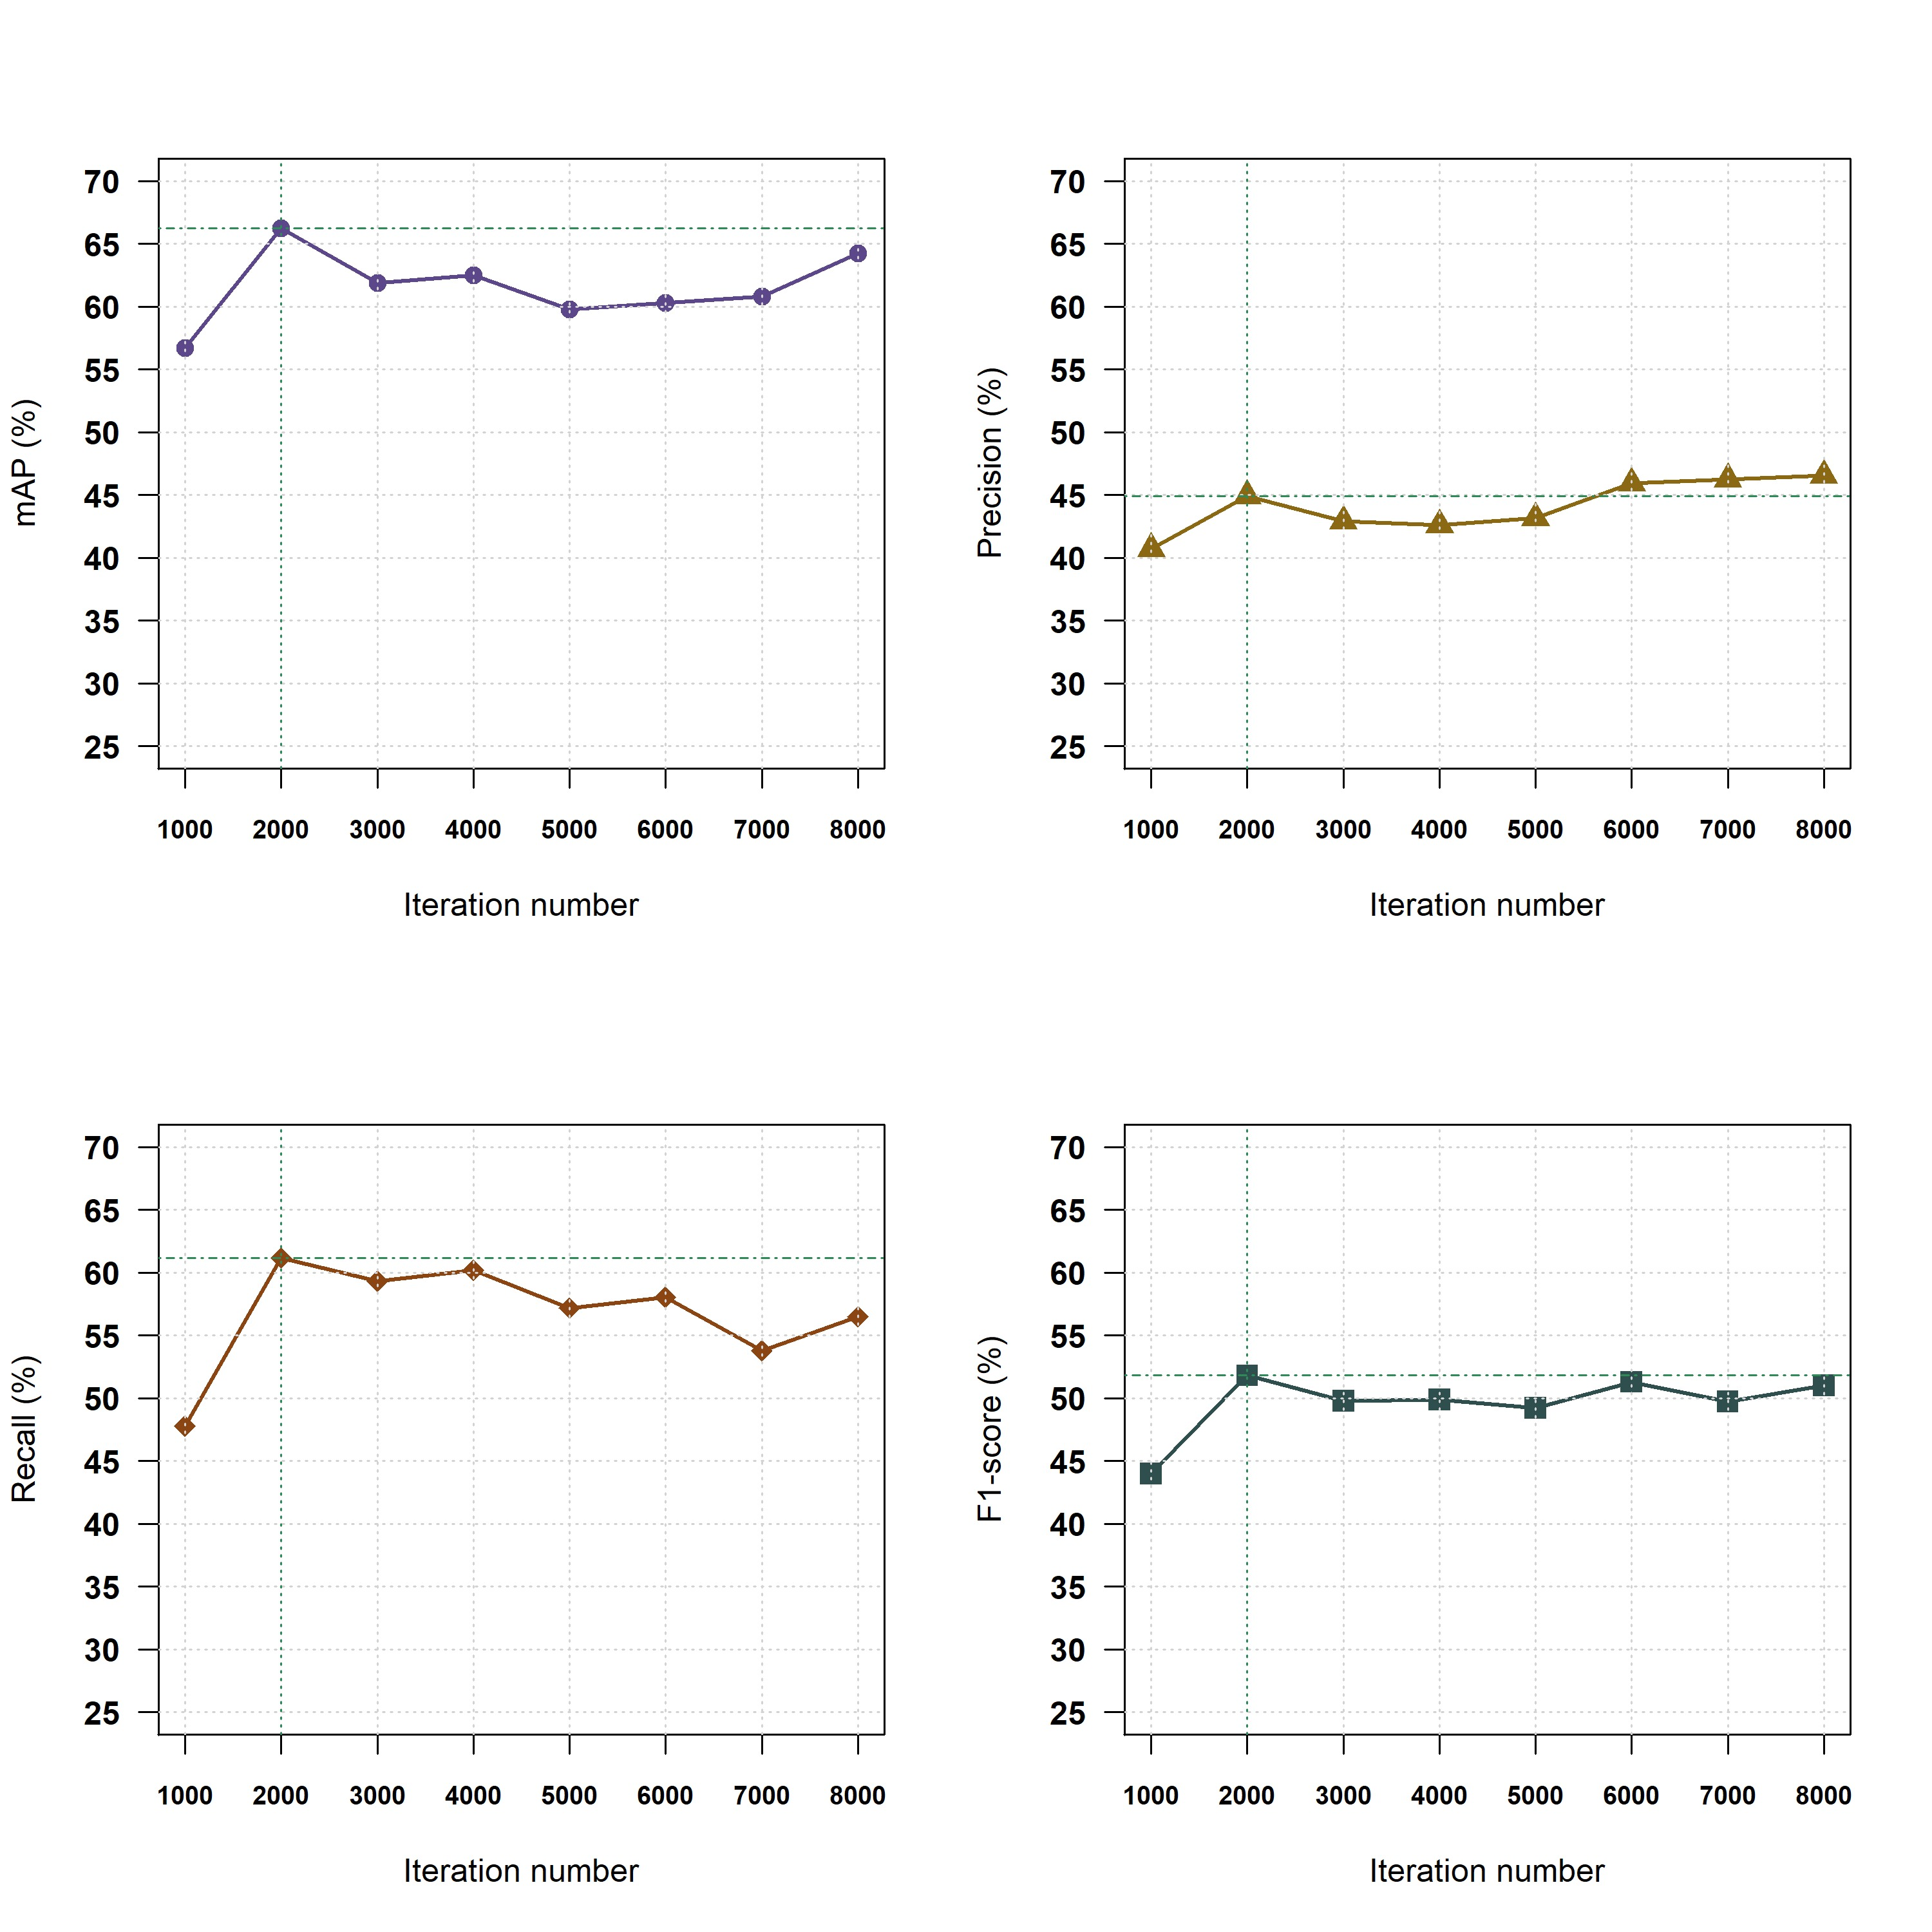
\includegraphics[width=0.85\textwidth]{img/chapters/resultados/metricas/metrics-train1.png}
\caption{\label{fig:metrics-train1}Resumen métricas primer entrenamiento de la red neuronal con el dataset de OIDv4}
\end{figure}

\newpage

\begin{table}[ht]
\centering
\caption{Métricas de calidad en el segundo entrenamiento con OIDv4 [1]}
\label{tab:metricas-test2_1}
\begin{tabular}{lcccccc}
\hline
\textbf{Iterations} & \textbf{\begin{tabular}[c]{@{}c@{}}AP person\\ (\%)\end{tabular}} & \textbf{\begin{tabular}[c]{@{}c@{}}AP bags\\ (\%)\end{tabular}} & \textbf{TP person} & \textbf{TP bags} & \textbf{FP person} & \textbf{FP bags} \\ \hline
1.000               & 30,81                                                             & 21,61                                                           & 5.216              & 231               & 9.220              & 579              \\
2.000               & 38,38                                                             & 53,59                                                           & 6.542              & 362               & 11.789             & 354              \\
3.000               & 33,51                                                             & 68,56                                                           & 7.232              & 419               & 18.887             & 411              \\
4.000               & 41,31                                                             & 77,12                                                           & 7.105              & 427               & 11.397             & 222              \\
5.000               & 38,86                                                             & 75,78                                                           & 6.586              & 444               & 11.735             & 398              \\
6.000               & 36,29                                                             & 66,49                                                           & 6.556              & 426               & 12.506             & 537              \\
7.000               & 39,94                                                             & 67,78                                                           & 6.246              & 418               & 9.744              & 523              \\
8.000               & 31,69                                                             & 69,07                                                           & 6.082              & 417               & 13.353             & 422              \\
9.000               & 43,34                                                             & 78,37                                                           & 6.773              & 451               & 9.846              & 373              \\
\textbf{10.000}     & \textbf{43,40}                                                    & \textbf{78,53}                                                  & \textbf{6.174}     & \textbf{426}      & \textbf{7.149}     & \textbf{217}     \\
11.000              & 38,81                                                             & 76,60                                                           & 7.166              & 446               & 12.162             & 387              \\
12.000              & 41,72                                                             & 78,10                                                           & 6.926              & 444               & 10.387             & 289              \\
13.000              & 39,48                                                             & 74,67                                                           & 6.575              & 406               & 9.850              & 238              \\
14.000              & 41,85                                                             & 73,69                                                           & 6.844              & 432               & 10.092             & 385              \\
15.000              & 40,19                                                             & 75,37                                                           & 6.915              & 423               & 11.426             & 252              \\
16.000              & 41,26                                                             & 75,17                                                           & 6.661              & 423               & 9.330              & 219              \\
17.000              & 42,13                                                             & 78,77                                                           & 6.991              & 433               & 9.924              & 242              \\
18.000              & 40,97                                                             & 75,45                                                           & 6.871              & 432               & 10.243             & 300              \\
19.000              & 39,01                                                             & 73,23                                                           & 6.822              & 428               & 10.791             & 333              \\
20.000              & 41,37                                                             & 78,38                                                           & 7.011              & 432               & 10.103             & 232              \\ \hline
\end{tabular}
\end{table}

\begin{table}[ht!]
\centering
\caption{Métricas de calidad en el segundo entrenamiento con OIDv4 [2]}
\label{tab:metricas-test2_2}
\begin{tabular}{lcccccccc}
\hline
\textbf{Iterations} & \textbf{TP}    & \textbf{FP}    & \textbf{FN}    & \textbf{\begin{tabular}[c]{@{}c@{}}Precision\\ (\%)\end{tabular}} & \textbf{\begin{tabular}[c]{@{}c@{}}Recall\\ (\%)\end{tabular}} & \textbf{\begin{tabular}[c]{@{}c@{}}F-score\\ (\%)\end{tabular}} & \textbf{\begin{tabular}[c]{@{}c@{}}Average\\ IoU (\%)\end{tabular}} & \textbf{\begin{tabular}[c]{@{}c@{}}mAP @ 0.5\\ (\%)\end{tabular}} \\ \hline
1.000               & 5.447          & 9.799          & 6.379          & 35,73                                                             & 46,06                                                          & 40,24                                                           & 25,72                                                               & 26,21                                                             \\
2.000               & 6.904          & 12.143         & 4.922          & 36,25                                                             & 58,38                                                          & 44,73                                                           & 27,30                                                               & 45,98                                                             \\
3.000               & 7.651          & 19.298         & 4.175          & 28,39                                                             & 64,70                                                          & 39,46                                                           & 21,66                                                               & 51,04                                                             \\
4.000               & 7.532          & 11.619         & 4.294          & 39,33                                                             & 63,69                                                          & 48,63                                                           & 30,90                                                               & 59,22                                                             \\
5.000               & 7.030          & 12.133         & 4.796          & 36,69                                                             & 59,45                                                          & 45,37                                                           & 28,28                                                               & 57,32                                                             \\
6.000               & 6.982          & 13.043         & 4.844          & 34,87                                                             & 59,04                                                          & 43,84                                                           & 27,23                                                               & 51,39                                                             \\
7.000               & 6.664          & 10.267         & 5.162          & 39,36                                                             & 56,35                                                          & 46,35                                                           & 30,96                                                               & 53,86                                                             \\
8.000               & 6.499          & 13.775         & 5.327          & 32,06                                                             & 54,96                                                          & 40,49                                                           & 24,96                                                               & 50,38                                                             \\
9.000               & 7.224          & 10.219         & 4.602          & 41,41                                                             & 61,09                                                          & 49,36                                                           & 32,95                                                               & 60,85                                                             \\
\textbf{10.000}     & \textbf{6.600} & \textbf{7.366} & \textbf{5.226} & \textbf{47,26}                                                    & \textbf{55,81}                                                 & \textbf{51,18}                                                  & \textbf{37,83}                                                      & \textbf{60,97}                                                    \\
11.000              & 7.612          & 12.549         & 4.214          & 37,76                                                             & 64,37                                                          & 47,59                                                           & 30,20                                                               & 57,70                                                             \\
12.000              & 7.370          & 10.676         & 4.456          & 40,84                                                             & 62,32                                                          & 49,34                                                           & 32,34                                                               & 59,91                                                             \\
13.000              & 6.981          & 10.088         & 4.845          & 40,90                                                             & 59,03                                                          & 48,32                                                           & 32,83                                                               & 57,07                                                             \\
14.000              & 7.276          & 10.477         & 4.550          & 40,98                                                             & 61,53                                                          & 49,20                                                           & 32,61                                                               & 57,77                                                             \\
15.000              & 7.338          & 11.678         & 4.488          & 38,59                                                             & 62,05                                                          & 47,58                                                           & 30,53                                                               & 57,78                                                             \\
16.000              & 7.084          & 9.549          & 4.742          & 42,59                                                             & 59,90                                                          & 49,78                                                           & 33,87                                                               & 58,22                                                             \\
17.000              & 7.424          & 10.166         & 4.402          & 42,21                                                             & 62,78                                                          & 50,48                                                           & 34,53                                                               & 60,45                                                             \\
18.000              & 7.303          & 10.543         & 4.523          & 40,92                                                             & 61,75                                                          & 49,22                                                           & 33,11                                                               & 58,21                                                             \\
19.000              & 7.250          & 11.124         & 4.576          & 39,46                                                             & 61,31                                                          & 48,01                                                           & 31,90                                                               & 56,12                                                             \\
20.000              & 7.443          & 10.335         & 4.383          & 41,87                                                             & 62,94                                                          & 50,28                                                           & 34,35                                                               & 59,93                                                             \\ \hline
\end{tabular}
\end{table}

\newpage

\begin{figure}[ht]
\centering
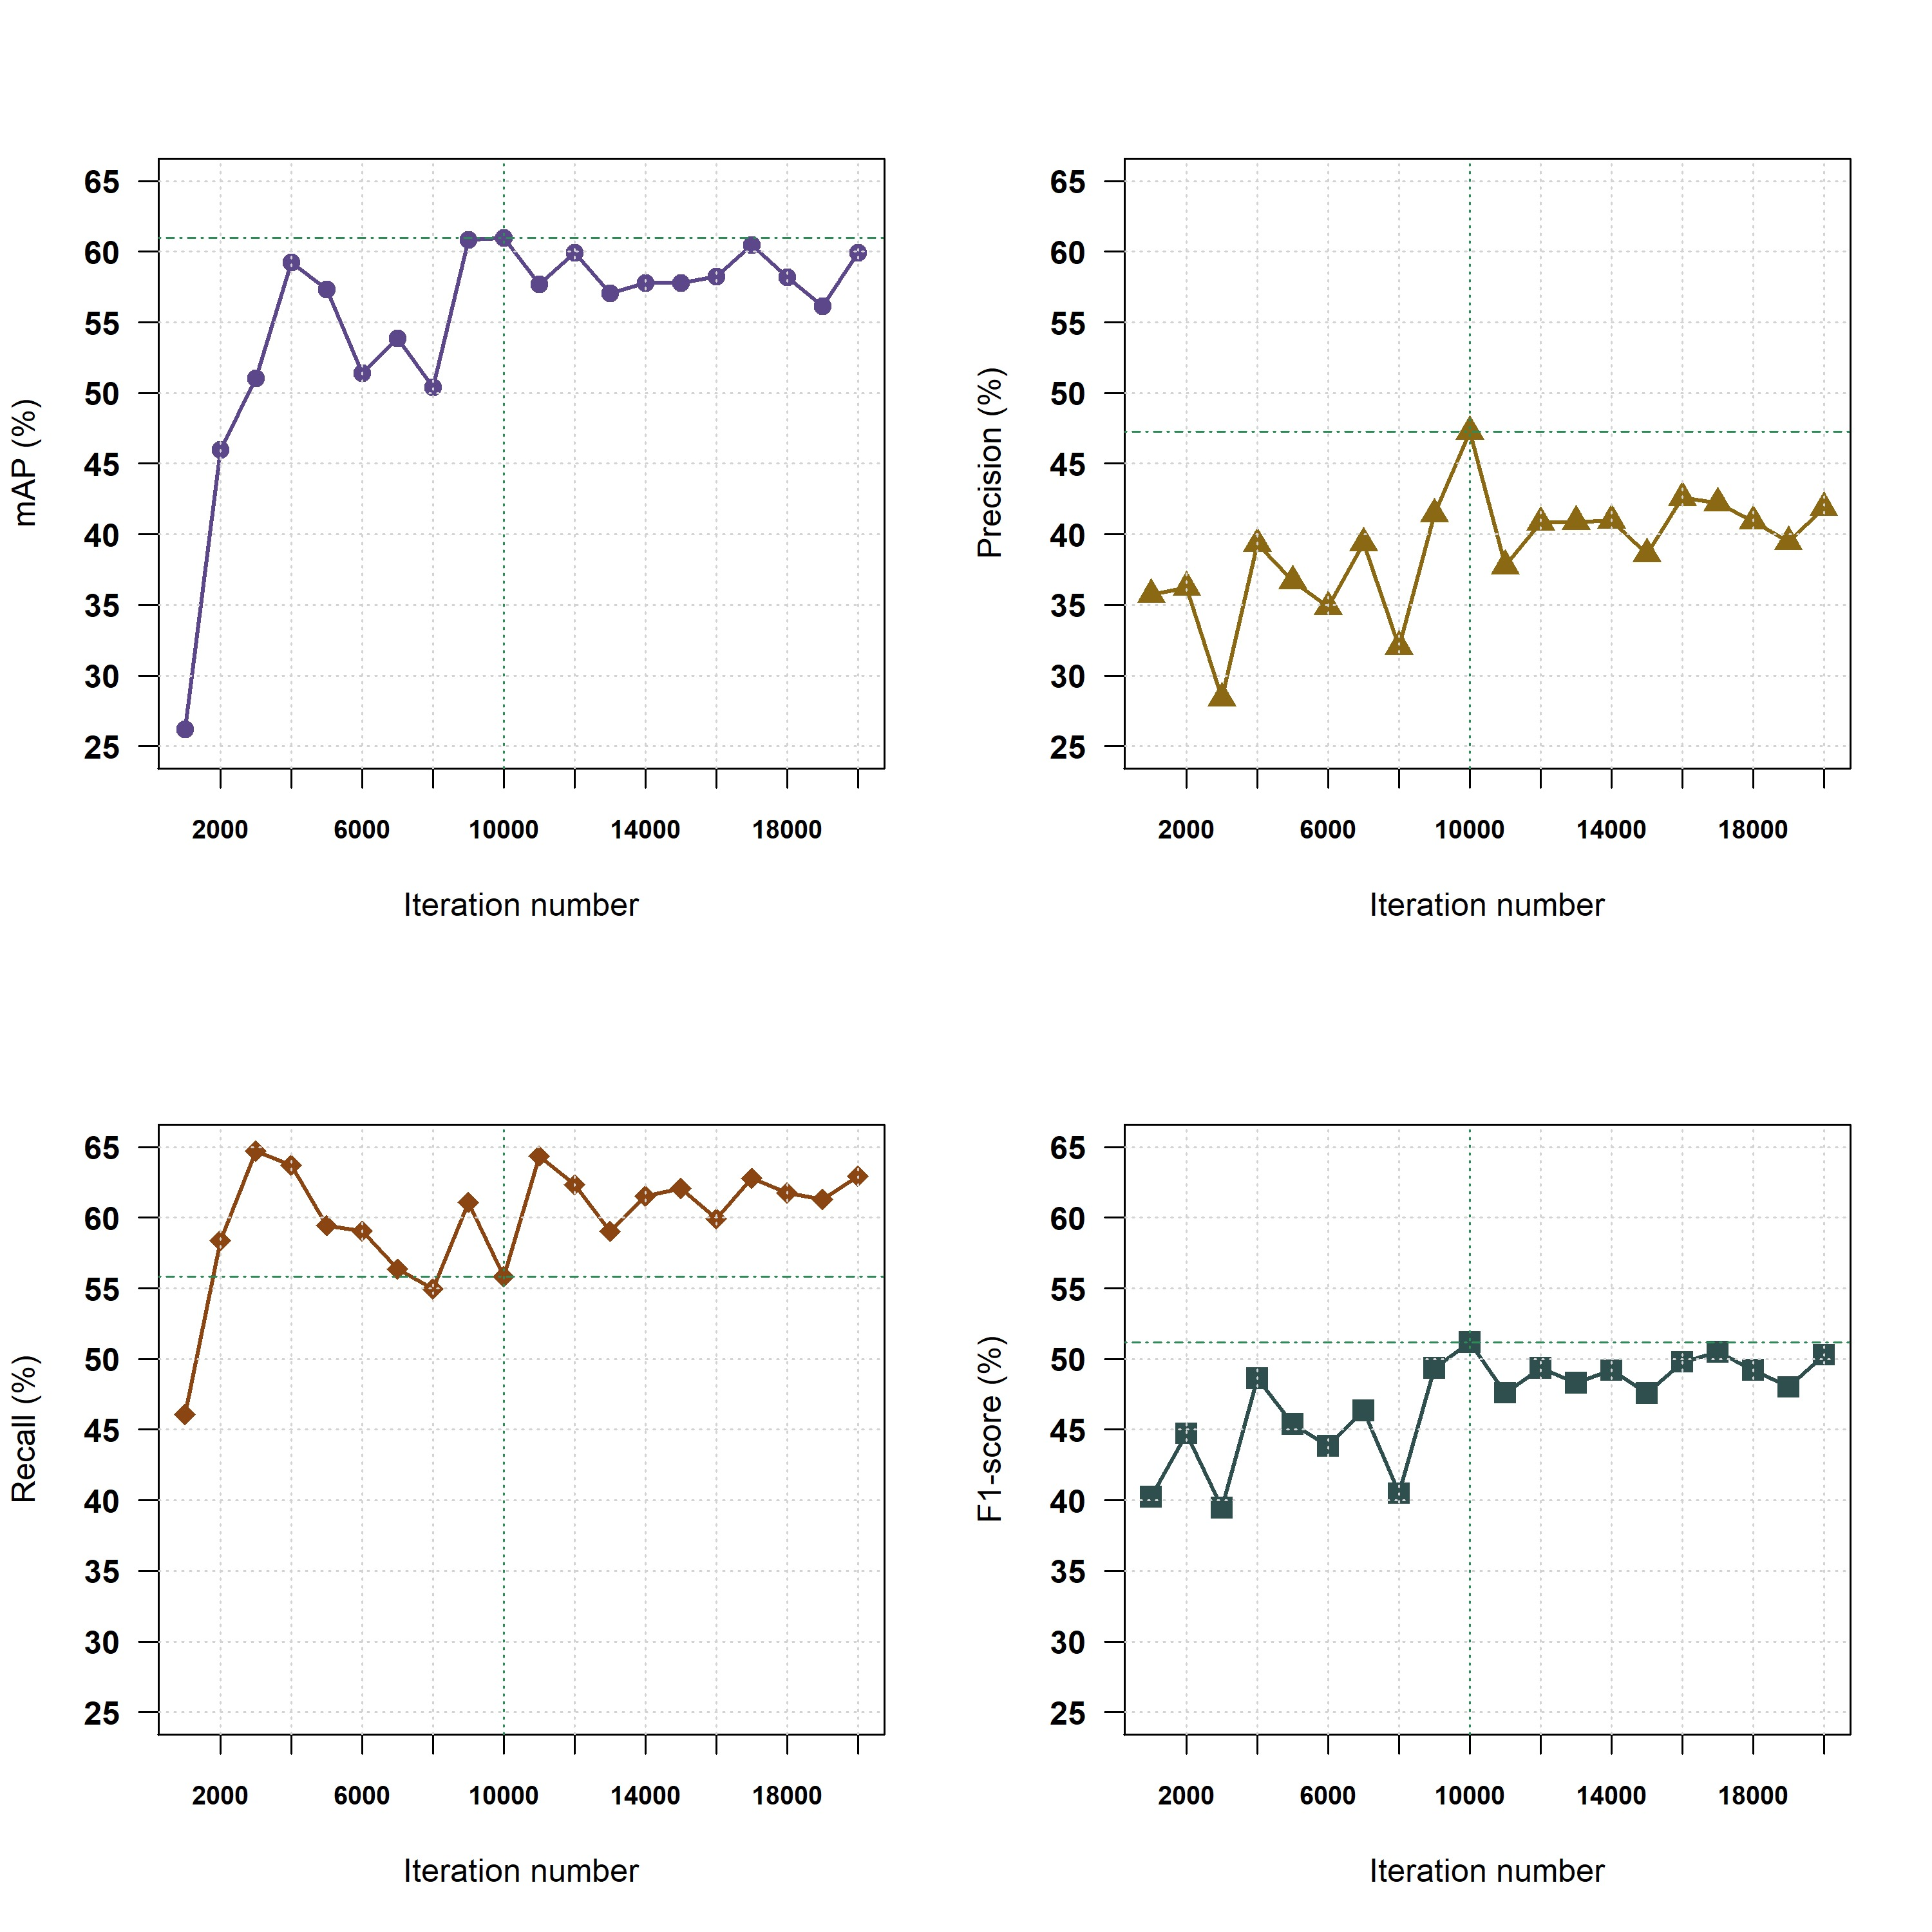
\includegraphics[width=0.85\textwidth]{img/chapters/resultados/metricas/metrics-train2.png}
\caption{\label{fig:metrics-train2}Resumen métricas segundo entrenamiento de la red neuronal con el dataset de OIDv4}
\end{figure}

\newpage

\subsection{Métricas de calidad en MS COCO Dataset}
\label{subsec:metricas-calidad-coco}

\begin{table}[ht]
\centering
\caption{Métricas de calidad de MS COCO en las clases de interés}
\label{tab:metricas-clases-coco}
\begin{tabular}{lccc}
\hline
\textbf{Class} & \textbf{AP(\%)} & \textbf{TP} & \textbf{FP} \\ \hline
Person         & 79,53           & 7.923       & 3.168       \\
Backpack       & 44,10           & 172         & 156         \\
Handbag        & 29,83           & 158         & 215         \\
Suitcase       & 71,08           & 205         & 102         \\ \hline
\end{tabular}
\end{table}

\begin{table}[ht]
\centering
\caption{Comparativa métricas de calidad entre los test en OIDv4 y MS COCO [1]}
\label{tab:comparativa-metricas1}
\begin{tabular}{lccc}
\hline
\textbf{Dataset}                   & \textbf{TP}          & \textbf{FP}          & \textbf{FN}          \\ \hline
\textbf{MS COCO}                   & \textbf{22.730}      & \textbf{10.889}      & \textbf{13.027}      \\
OIDv4 test 1                       & 430                  & 527                  & 273                  \\
OIDv4 test 2                       & 6.600                & 7.366                & 5.226                \\ \hline
\end{tabular}
\end{table}

\begin{table}[ht]
\centering
\caption{Comparativa métricas de calidad entre los dos test en OIDv4 y MS COCO [2]}
\label{tab:comparativa-metricas2}
\begin{tabular}{cccccc}
\hline
\rowcolor[HTML]{FFFFFF} 
\textbf{Dataset}             & \textbf{\begin{tabular}[c]{@{}c@{}}Precision\\ (\%)\end{tabular}} & \textbf{\begin{tabular}[c]{@{}c@{}}Recall\\ (\%)\end{tabular}} & \textbf{\begin{tabular}[c]{@{}c@{}}F-score\\ (\%)\end{tabular}} & \textbf{\begin{tabular}[c]{@{}c@{}}average IoU\\ (\%)\end{tabular}} & \textbf{\begin{tabular}[c]{@{}c@{}}mAP @ 0.5\\ (\%)\end{tabular}} \\ \hline
\textbf{MS COCO}             & \textbf{67,61}                                                    & \textbf{63,57}                                                 & \textbf{65,53}                                                  & \textbf{56.04}                                                      & \textbf{64.16}                                                    \\
OIDv4 test 1                 & 44,93                                                             & 61,17                                                          & 51,81                                                           & 34,13                                                               & 66,25                                                             \\
OIDv4 test 2                 & 47,26                                                             & 55,81                                                          & 51,18                                                           & 37,83                                                               & 60,97                                                             \\ \hline
\end{tabular}
\end{table}

\newpage

\subsection{Resultados en detección de objetos y personas con YOLOv4}
\label{subsec:resultados-yolov4-tf}

\textcolor{red}{Poner imágenes de las detecciones en los datasets empleados y explicar con detalle como influye distintos elementos como la distancia, iluminación, color, etc... en la detección de objetos}.

\url{https://old.photojoiner.net/}

\textcolor{red}{También hacer tablas durante un número determinado de fotogramas donde, a modo de ejemplo se calcule las métricas más relevantes}.

\newpage

\subsection{Resultados en seguimiento de objetos y personas con YOLOv4 y Deep SORT}
\label{subsec:resultados-yolov4+deepsort}

\textcolor{red}{Poner imágenes de las detecciones en los datasets empleados y explicar con detalle los problemas con los que nos podemos encontrar a la hora de hacer un seguimiento o \textit{tracking} de objetos y personas, se pierde el rastreo y se vuelve a asociar una nueva ID a ese individuo, también explicar que debido al \textit{threshold} que pongamos se pueden perder objetos, pero tampoco es conveniente bajarlo a más de X porque entonces se confunden objetos o se trackean varias veces}.

\newpage

\subsection{Resultados en algoritmo de detección de objetos abandonados}
\label{subsec:resultados-abandon-algorithm}

\textcolor{red}{Poner ejemplos de avssab2007easy (warning + abandoned), avssab2007medium (sin asignacion de propietario), aboda (warning + abandoned), gba (warning + abandoned), pets2007 y alguno de gba problemas de con cambios de identidad con lo que es imposible trackear un objeto}

\begin{figure}[ht]
\centering
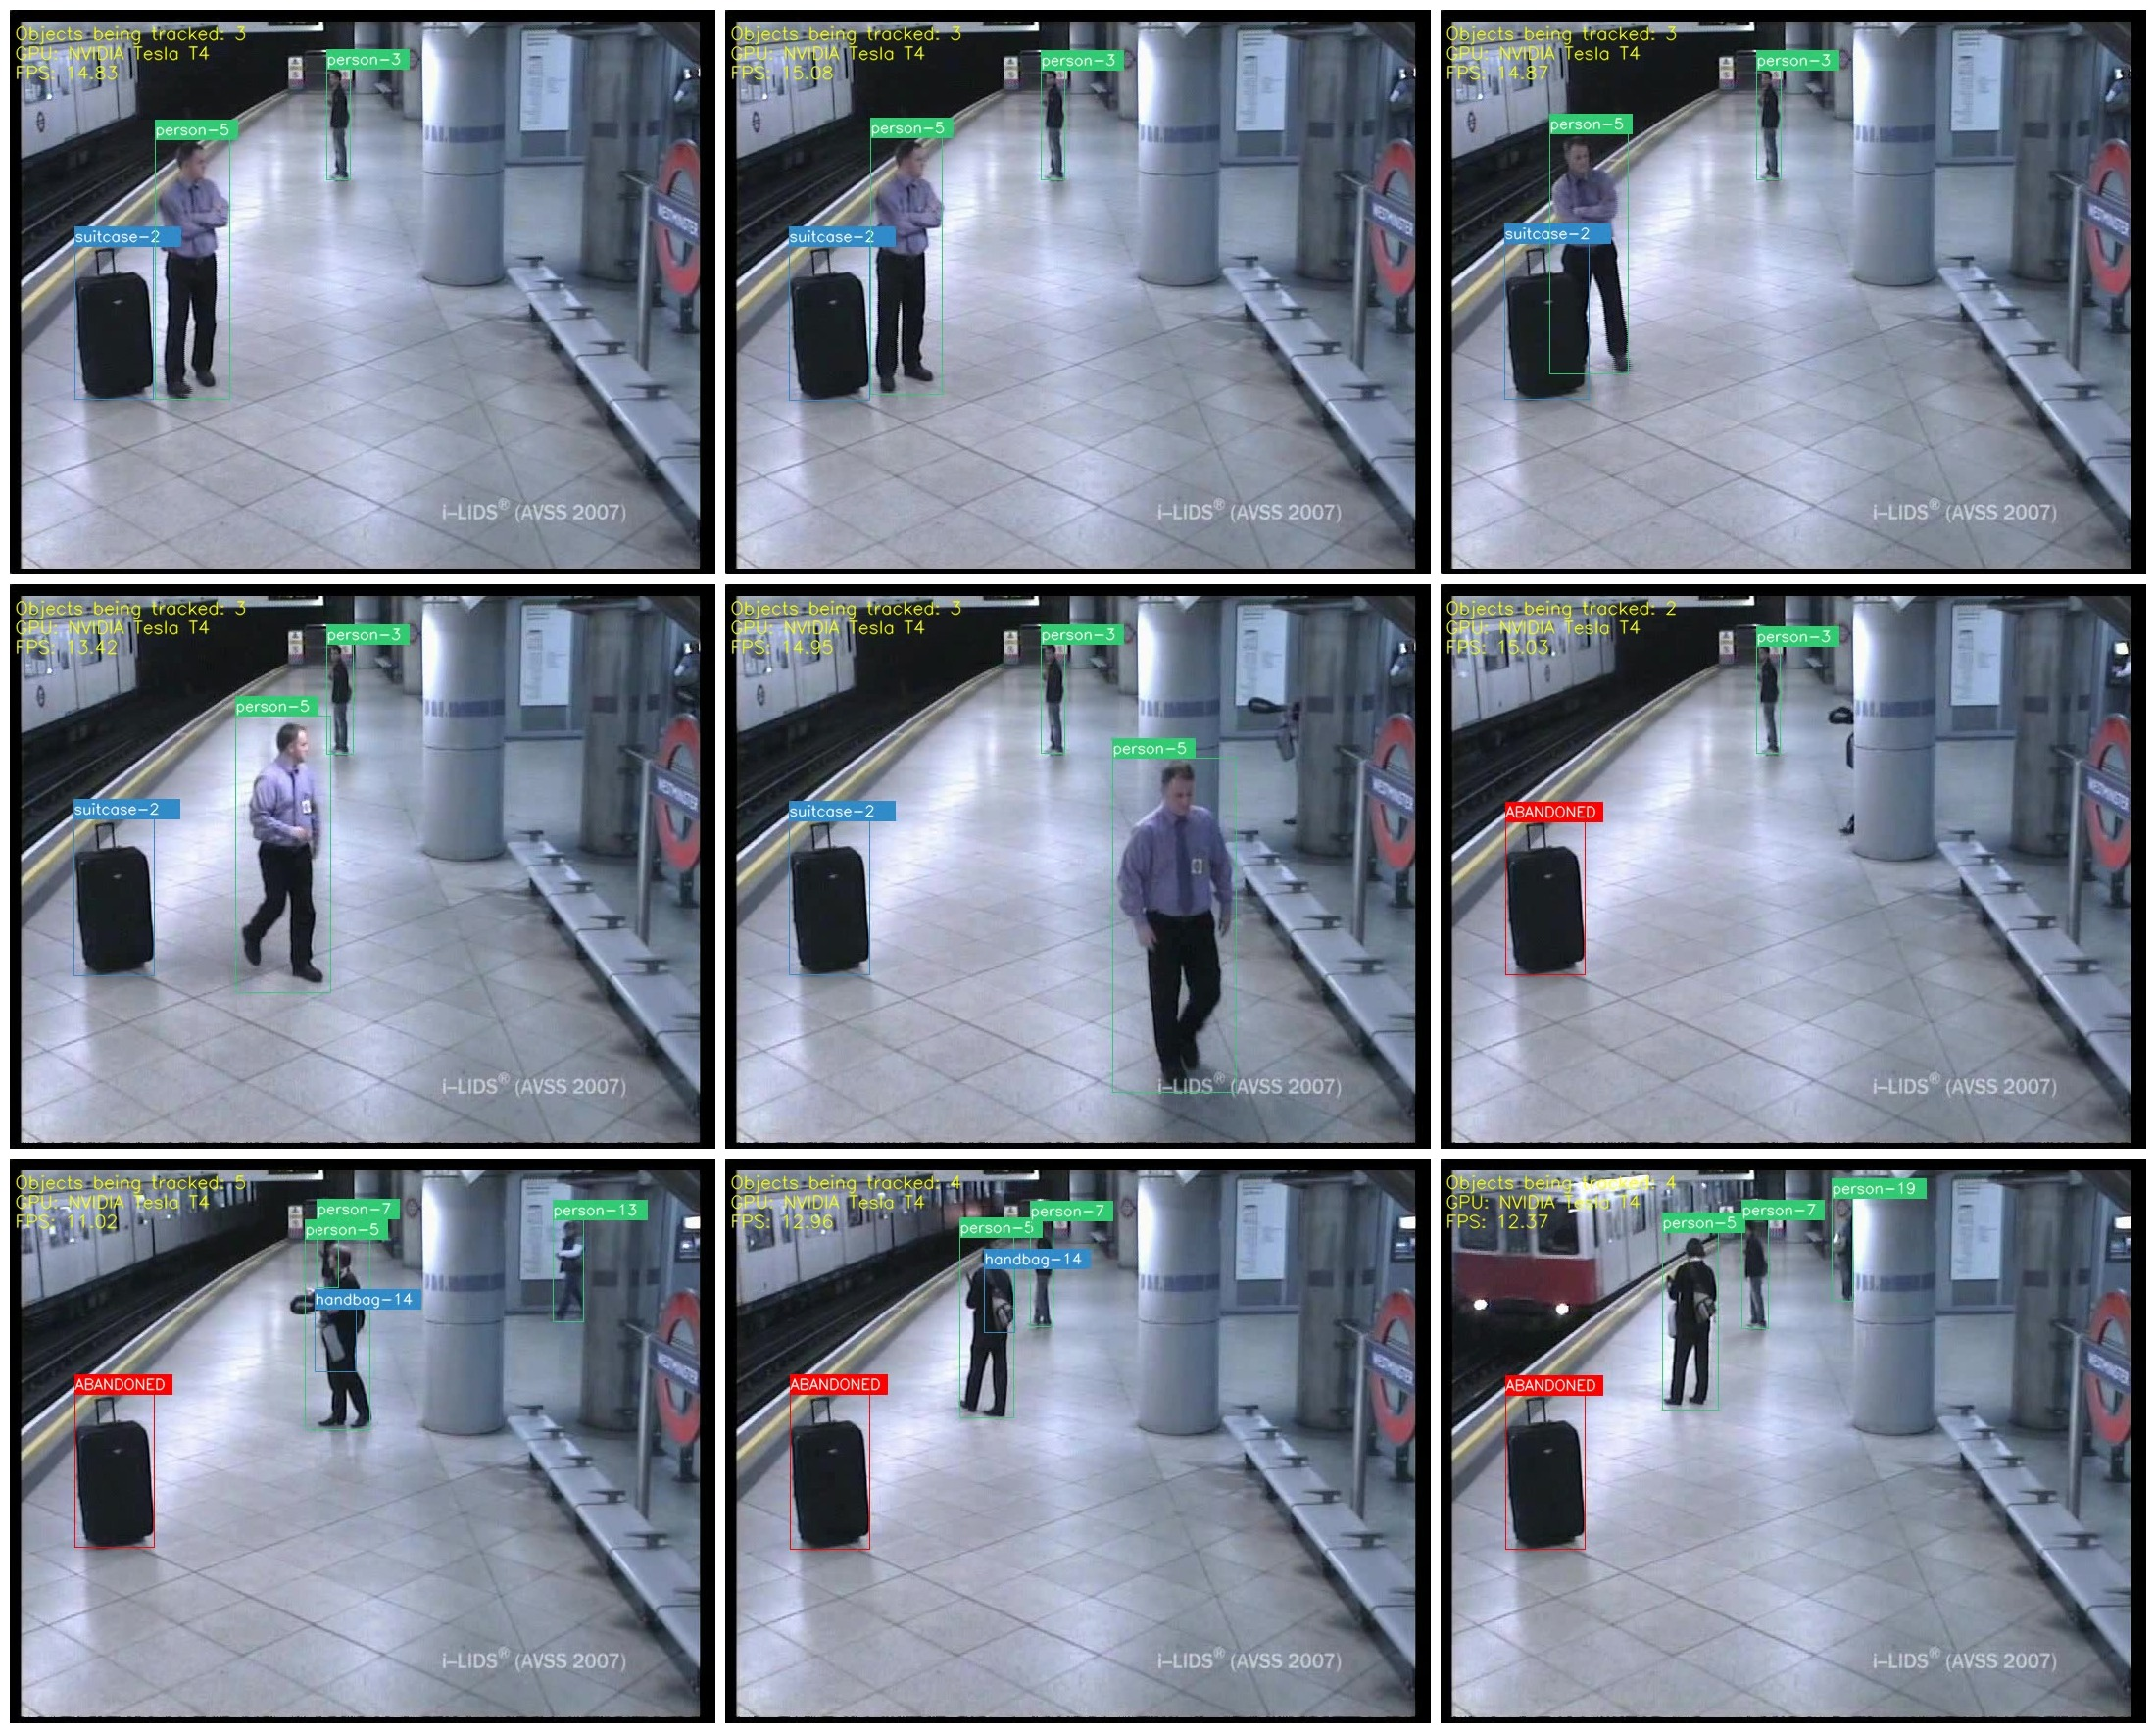
\includegraphics[width=0.85\textwidth]{img/chapters/resultados/abandono/abandoned-avssab2007-example2.png}
\caption{\label{fig:propietario-desaparece-plano}Propietario maleta desaparece del plano de visión}
\end{figure}

\textcolor{red}{Aquí meter un subsubapartado con métricas relevantes en la detección de objetos abandonados}.

\newpage

\section{Conclusiones}
\label{sec:conclu-resultados}

